% Options for packages loaded elsewhere
\PassOptionsToPackage{unicode}{hyperref}
\PassOptionsToPackage{hyphens}{url}
\PassOptionsToPackage{dvipsnames,svgnames,x11names}{xcolor}
%
\documentclass[
  letterpaper,
  DIV=11,
  numbers=noendperiod]{scrartcl}

\usepackage{amsmath,amssymb}
\usepackage{iftex}
\ifPDFTeX
  \usepackage[T1]{fontenc}
  \usepackage[utf8]{inputenc}
  \usepackage{textcomp} % provide euro and other symbols
\else % if luatex or xetex
  \usepackage{unicode-math}
  \defaultfontfeatures{Scale=MatchLowercase}
  \defaultfontfeatures[\rmfamily]{Ligatures=TeX,Scale=1}
\fi
\usepackage{lmodern}
\ifPDFTeX\else  
    % xetex/luatex font selection
\fi
% Use upquote if available, for straight quotes in verbatim environments
\IfFileExists{upquote.sty}{\usepackage{upquote}}{}
\IfFileExists{microtype.sty}{% use microtype if available
  \usepackage[]{microtype}
  \UseMicrotypeSet[protrusion]{basicmath} % disable protrusion for tt fonts
}{}
\makeatletter
\@ifundefined{KOMAClassName}{% if non-KOMA class
  \IfFileExists{parskip.sty}{%
    \usepackage{parskip}
  }{% else
    \setlength{\parindent}{0pt}
    \setlength{\parskip}{6pt plus 2pt minus 1pt}}
}{% if KOMA class
  \KOMAoptions{parskip=half}}
\makeatother
\usepackage{xcolor}
\setlength{\emergencystretch}{3em} % prevent overfull lines
\setcounter{secnumdepth}{-\maxdimen} % remove section numbering
% Make \paragraph and \subparagraph free-standing
\makeatletter
\ifx\paragraph\undefined\else
  \let\oldparagraph\paragraph
  \renewcommand{\paragraph}{
    \@ifstar
      \xxxParagraphStar
      \xxxParagraphNoStar
  }
  \newcommand{\xxxParagraphStar}[1]{\oldparagraph*{#1}\mbox{}}
  \newcommand{\xxxParagraphNoStar}[1]{\oldparagraph{#1}\mbox{}}
\fi
\ifx\subparagraph\undefined\else
  \let\oldsubparagraph\subparagraph
  \renewcommand{\subparagraph}{
    \@ifstar
      \xxxSubParagraphStar
      \xxxSubParagraphNoStar
  }
  \newcommand{\xxxSubParagraphStar}[1]{\oldsubparagraph*{#1}\mbox{}}
  \newcommand{\xxxSubParagraphNoStar}[1]{\oldsubparagraph{#1}\mbox{}}
\fi
\makeatother

\usepackage{color}
\usepackage{fancyvrb}
\newcommand{\VerbBar}{|}
\newcommand{\VERB}{\Verb[commandchars=\\\{\}]}
\DefineVerbatimEnvironment{Highlighting}{Verbatim}{commandchars=\\\{\}}
% Add ',fontsize=\small' for more characters per line
\usepackage{framed}
\definecolor{shadecolor}{RGB}{241,243,245}
\newenvironment{Shaded}{\begin{snugshade}}{\end{snugshade}}
\newcommand{\AlertTok}[1]{\textcolor[rgb]{0.68,0.00,0.00}{#1}}
\newcommand{\AnnotationTok}[1]{\textcolor[rgb]{0.37,0.37,0.37}{#1}}
\newcommand{\AttributeTok}[1]{\textcolor[rgb]{0.40,0.45,0.13}{#1}}
\newcommand{\BaseNTok}[1]{\textcolor[rgb]{0.68,0.00,0.00}{#1}}
\newcommand{\BuiltInTok}[1]{\textcolor[rgb]{0.00,0.23,0.31}{#1}}
\newcommand{\CharTok}[1]{\textcolor[rgb]{0.13,0.47,0.30}{#1}}
\newcommand{\CommentTok}[1]{\textcolor[rgb]{0.37,0.37,0.37}{#1}}
\newcommand{\CommentVarTok}[1]{\textcolor[rgb]{0.37,0.37,0.37}{\textit{#1}}}
\newcommand{\ConstantTok}[1]{\textcolor[rgb]{0.56,0.35,0.01}{#1}}
\newcommand{\ControlFlowTok}[1]{\textcolor[rgb]{0.00,0.23,0.31}{\textbf{#1}}}
\newcommand{\DataTypeTok}[1]{\textcolor[rgb]{0.68,0.00,0.00}{#1}}
\newcommand{\DecValTok}[1]{\textcolor[rgb]{0.68,0.00,0.00}{#1}}
\newcommand{\DocumentationTok}[1]{\textcolor[rgb]{0.37,0.37,0.37}{\textit{#1}}}
\newcommand{\ErrorTok}[1]{\textcolor[rgb]{0.68,0.00,0.00}{#1}}
\newcommand{\ExtensionTok}[1]{\textcolor[rgb]{0.00,0.23,0.31}{#1}}
\newcommand{\FloatTok}[1]{\textcolor[rgb]{0.68,0.00,0.00}{#1}}
\newcommand{\FunctionTok}[1]{\textcolor[rgb]{0.28,0.35,0.67}{#1}}
\newcommand{\ImportTok}[1]{\textcolor[rgb]{0.00,0.46,0.62}{#1}}
\newcommand{\InformationTok}[1]{\textcolor[rgb]{0.37,0.37,0.37}{#1}}
\newcommand{\KeywordTok}[1]{\textcolor[rgb]{0.00,0.23,0.31}{\textbf{#1}}}
\newcommand{\NormalTok}[1]{\textcolor[rgb]{0.00,0.23,0.31}{#1}}
\newcommand{\OperatorTok}[1]{\textcolor[rgb]{0.37,0.37,0.37}{#1}}
\newcommand{\OtherTok}[1]{\textcolor[rgb]{0.00,0.23,0.31}{#1}}
\newcommand{\PreprocessorTok}[1]{\textcolor[rgb]{0.68,0.00,0.00}{#1}}
\newcommand{\RegionMarkerTok}[1]{\textcolor[rgb]{0.00,0.23,0.31}{#1}}
\newcommand{\SpecialCharTok}[1]{\textcolor[rgb]{0.37,0.37,0.37}{#1}}
\newcommand{\SpecialStringTok}[1]{\textcolor[rgb]{0.13,0.47,0.30}{#1}}
\newcommand{\StringTok}[1]{\textcolor[rgb]{0.13,0.47,0.30}{#1}}
\newcommand{\VariableTok}[1]{\textcolor[rgb]{0.07,0.07,0.07}{#1}}
\newcommand{\VerbatimStringTok}[1]{\textcolor[rgb]{0.13,0.47,0.30}{#1}}
\newcommand{\WarningTok}[1]{\textcolor[rgb]{0.37,0.37,0.37}{\textit{#1}}}

\providecommand{\tightlist}{%
  \setlength{\itemsep}{0pt}\setlength{\parskip}{0pt}}\usepackage{longtable,booktabs,array}
\usepackage{calc} % for calculating minipage widths
% Correct order of tables after \paragraph or \subparagraph
\usepackage{etoolbox}
\makeatletter
\patchcmd\longtable{\par}{\if@noskipsec\mbox{}\fi\par}{}{}
\makeatother
% Allow footnotes in longtable head/foot
\IfFileExists{footnotehyper.sty}{\usepackage{footnotehyper}}{\usepackage{footnote}}
\makesavenoteenv{longtable}
\usepackage{graphicx}
\makeatletter
\newsavebox\pandoc@box
\newcommand*\pandocbounded[1]{% scales image to fit in text height/width
  \sbox\pandoc@box{#1}%
  \Gscale@div\@tempa{\textheight}{\dimexpr\ht\pandoc@box+\dp\pandoc@box\relax}%
  \Gscale@div\@tempb{\linewidth}{\wd\pandoc@box}%
  \ifdim\@tempb\p@<\@tempa\p@\let\@tempa\@tempb\fi% select the smaller of both
  \ifdim\@tempa\p@<\p@\scalebox{\@tempa}{\usebox\pandoc@box}%
  \else\usebox{\pandoc@box}%
  \fi%
}
% Set default figure placement to htbp
\def\fps@figure{htbp}
\makeatother

\KOMAoption{captions}{tableheading}
\makeatletter
\@ifpackageloaded{caption}{}{\usepackage{caption}}
\AtBeginDocument{%
\ifdefined\contentsname
  \renewcommand*\contentsname{Table of contents}
\else
  \newcommand\contentsname{Table of contents}
\fi
\ifdefined\listfigurename
  \renewcommand*\listfigurename{List of Figures}
\else
  \newcommand\listfigurename{List of Figures}
\fi
\ifdefined\listtablename
  \renewcommand*\listtablename{List of Tables}
\else
  \newcommand\listtablename{List of Tables}
\fi
\ifdefined\figurename
  \renewcommand*\figurename{Figure}
\else
  \newcommand\figurename{Figure}
\fi
\ifdefined\tablename
  \renewcommand*\tablename{Table}
\else
  \newcommand\tablename{Table}
\fi
}
\@ifpackageloaded{float}{}{\usepackage{float}}
\floatstyle{ruled}
\@ifundefined{c@chapter}{\newfloat{codelisting}{h}{lop}}{\newfloat{codelisting}{h}{lop}[chapter]}
\floatname{codelisting}{Listing}
\newcommand*\listoflistings{\listof{codelisting}{List of Listings}}
\makeatother
\makeatletter
\makeatother
\makeatletter
\@ifpackageloaded{caption}{}{\usepackage{caption}}
\@ifpackageloaded{subcaption}{}{\usepackage{subcaption}}
\makeatother

\usepackage{bookmark}

\IfFileExists{xurl.sty}{\usepackage{xurl}}{} % add URL line breaks if available
\urlstyle{same} % disable monospaced font for URLs
\hypersetup{
  pdftitle={K-Nearest Neighbours},
  pdfauthor={Ondřej Duba; Filip Molhanec},
  colorlinks=true,
  linkcolor={blue},
  filecolor={Maroon},
  citecolor={Blue},
  urlcolor={Blue},
  pdfcreator={LaTeX via pandoc}}


\title{K-Nearest Neighbours}
\author{Ondřej Duba \and Filip Molhanec}
\date{2025-01-10}

\begin{document}
\maketitle


\section{What is KNN}\label{what-is-knn}

Although K-Nearest Neigbours (KNN) is often regarded as very simple
machine learning algorithm, its utility and power are undeniable. It is
one of the core algorithms for supervised learning. Simply put,
supervised learning is proccess of creating model that can predict value
of target variable based on input data, using knowledge from dataset
where we know the actual values of the target variables. KNN can be
effectively used for both classification (target variable can take a
limited number of values) and regression (target variable can take on
continuous range of values) tasks. The simplest explanation of KNN for
classification tasks is that an object is classifed by plurality vote of
its \emph{k} nearest neighbours. For regression tasks, KNN can be
generalized so that an object is assigned value that is the average of
the values of its \emph{k} nearest neigbours. However, this is just a
basic overview and there are several factors to consider when using KNN
to develop an effective machine learning model.

```roaqn latex

\section{What is KNN?}

Although K-Nearest Neigbours (KNN) is often regarded as very simple
machine learning algorithm, its utility and power are undeniable. It is
one of the core algorithms for supervised learning. Simply put,
supervised learning is proccess of creating model that can predict value
of target variable based on input data, using knowledge from dataset
where we know the actual values of the target variables. KNN can be
effectively used for both classification (target variable can take a
limited number of values) and regression (target variable can take on
continuous range of values) tasks. The simplest explanation of KNN for
classification tasks is that an object is classifed by plurality vote of
its k nearest neighbours. For regression tasks, KNN can be generalized
so that an object is assigned value that is the average of the values of
its k nearest neigbours. However, this is just a basic overview and
there are several factors to consider when using KNN to develop an
effective machine learning model.

\textbackslash end\{document\}```

\section{Dataset description}\label{dataset-description}

We have chosen
\href{https://www.kaggle.com/datasets/mujtabamatin/air-quality-and-pollution-assessment/data}{\emph{Air
Quality and Pollution Assesment}} dataset to show how K-Nearest
Neighbours algorithm works. This Dataset is derived from
\href{https://www.who.int/health-topics/air-pollution\#tab=tab_1}{World
Health Organization} and
\href{https://data.worldbank.org/indicator/EN.POP.DNST}{World Bank
Group} This Dataset contains several features, in other words, columns,
lets go through each one of them and explain what they mean.

\begin{itemize}
\tightlist
\item
  \textbf{Temperature(°C)}: Average temperature of the region
\item
  \textbf{Humidity (\%)}: Relative humidity recorded in the region
\item
  \textbf{PM2.5 Concentration (µg/m³)}: Fine particulate matter level
\item
  \textbf{PM10 Concentration (µg/m³)}: Coarse particulate matter levels
\item
  \textbf{NO2 Concentration (ppb)}: Nitrogen dioxide levels
\item
  \textbf{SO2 Concentration (ppb)}: Sulfur dioxide levels
\item
  \textbf{CO Concentration (ppm)}: Carbon monoxide levels
\item
  \textbf{Proximity to Industrial Areas (km)}: Distance to the nearest
  industrial zone
\item
  \textbf{Population Density (people/km²)}: Number of people per square
  kilometer in the region
\end{itemize}

Then there is so called Target Variable, that's the variable that we are
trying to predict, in our dataset, it is called \textbf{Air Quality} and
it can have 4 possible values depending on Air Quality, these values are
the following:

\begin{itemize}
\tightlist
\item
  \textbf{Good}: Clean air with low pollution levels.
\item
  \textbf{Moderate}: Acceptable air quality but with some pollutants
  present.
\item
  \textbf{Poor}: Noticeable pollution that may cause health issues for
  sensitive groups.
\item
  \textbf{Hazardous}: Highly polluted air posing serious health risks to
  the population.n.
\end{itemize}

\section{Importing all libraries that will be
used}\label{importing-all-libraries-that-will-be-used}

\section{Preprocessing data}\label{preprocessing-data}

As part of data preprocessing we read data from csv file and then we
preprocess them. Considering that there are no missing values, there is
no need to fill them. All features are already numerical, so there is no
need to convert them any further. Target variable can take on 4 values,
and there is order between those values (it is ordinal categorical
datatype), so we convert it into categorical type with order between
them. We split data into 3 parts, train, validate and test with train
size being 60\% of the original dataset and validate and test both being
20\% of the original dataset

\begin{Shaded}
\begin{Highlighting}[]
\KeywordTok{def}\NormalTok{ preprocess\_data(df:pd.DataFrame)}\OperatorTok{{-}\textgreater{}}\NormalTok{pd.DataFrame:}
    \CommentTok{""" Function, for preprocessing data}
\CommentTok{    """}
\NormalTok{    qual\_category }\OperatorTok{=}\NormalTok{ pd.api.types.CategoricalDtype(categories}\OperatorTok{=}\NormalTok{[}\StringTok{\textquotesingle{}Hazardous\textquotesingle{}}\NormalTok{, }\StringTok{\textquotesingle{}Poor\textquotesingle{}}\NormalTok{, }\StringTok{\textquotesingle{}Moderate\textquotesingle{}}\NormalTok{, }\StringTok{\textquotesingle{}Good\textquotesingle{}}\NormalTok{], ordered}\OperatorTok{=}\VariableTok{True}\NormalTok{)}
\NormalTok{    df[}\StringTok{\textquotesingle{}Air Quality\textquotesingle{}}\NormalTok{] }\OperatorTok{=}\NormalTok{ df[}\StringTok{\textquotesingle{}Air Quality\textquotesingle{}}\NormalTok{].astype(qual\_category)}
    \ControlFlowTok{return}\NormalTok{ df}
    
\end{Highlighting}
\end{Shaded}

\begin{Shaded}
\begin{Highlighting}[]
\KeywordTok{def}\NormalTok{ read\_data(path:}\BuiltInTok{str}\OperatorTok{=}\StringTok{\textquotesingle{}data/data.csv\textquotesingle{}}\NormalTok{, y:}\BuiltInTok{str}\OperatorTok{=}\StringTok{\textquotesingle{}Air Quality\textquotesingle{}}\NormalTok{,}\OperatorTok{**}\NormalTok{kwargs)}\OperatorTok{{-}\textgreater{}}\BuiltInTok{tuple}\NormalTok{:}
    \CommentTok{""" Function thats read data, and splits them into Train, Validation and Test datasets}
\CommentTok{    also separates, target value from others values.}
\CommentTok{    {-}{-}{-}}
\CommentTok{    Attributes:}
\CommentTok{    path: [str], path to csv data file}
\CommentTok{    y: [str], name of Target value}
\CommentTok{    kwargs: options, use seed for random\_seed}
\CommentTok{    {-}{-}{-}}
\CommentTok{    Returns:}
\CommentTok{    tuple with Train,Validation,Test parametrs set, Target values: Train, Test, Validation}
\CommentTok{    """}
\NormalTok{    df }\OperatorTok{=}\NormalTok{ pd.read\_csv(path)}

\NormalTok{    display(df.info())}
\NormalTok{    display(df.describe())}
    
\NormalTok{    df }\OperatorTok{=}\NormalTok{ preprocess\_data(df)}
    \CommentTok{\# Split the training dataset into train and rest (default 60\% : 40\%)}
\NormalTok{    Xtrain, Xrest, ytrain, yrest }\OperatorTok{=}\NormalTok{ train\_test\_split(}
\NormalTok{        df.drop(columns}\OperatorTok{=}\NormalTok{[y]), df[y], test\_size}\OperatorTok{=}\FloatTok{0.4}\NormalTok{, random\_state}\OperatorTok{=}\NormalTok{kwargs.get(}\StringTok{\textquotesingle{}seed\textquotesingle{}}\NormalTok{,}\DecValTok{42}\NormalTok{))}
    \CommentTok{\# Split the rest of the data into validation dataset and test dataset (default: 24\% : 16\%)}
\NormalTok{    Xtest, Xval, ytest, yval }\OperatorTok{=}\NormalTok{ train\_test\_split(}
\NormalTok{        Xrest, yrest, test\_size}\OperatorTok{=}\FloatTok{0.5}\NormalTok{, random\_state}\OperatorTok{=}\NormalTok{kwargs.get(}\StringTok{\textquotesingle{}seed\textquotesingle{}}\NormalTok{,}\DecValTok{42}\NormalTok{))}
    \BuiltInTok{print}\NormalTok{(}\SpecialStringTok{f\textquotesingle{}Dataset: }\SpecialCharTok{\{}\NormalTok{path}\SpecialCharTok{\}}\SpecialStringTok{ | Target value: }\SpecialCharTok{\{}\NormalTok{y}\SpecialCharTok{\}}\SpecialStringTok{ | Seed: }\SpecialCharTok{\{}\NormalTok{kwargs}\SpecialCharTok{.}\NormalTok{get(}\StringTok{\textquotesingle{}seed\textquotesingle{}}\NormalTok{,}\DecValTok{42}\NormalTok{)}\SpecialCharTok{\}}\SpecialStringTok{\textquotesingle{}}\NormalTok{)}
    \ControlFlowTok{return}\NormalTok{ Xtrain, Xtest, Xval, ytrain, ytest, yval}
\end{Highlighting}
\end{Shaded}

\begin{Shaded}
\begin{Highlighting}[]
\NormalTok{Xtrain, Xtest, Xval, ytrain, ytest, yval }\OperatorTok{=}\NormalTok{ read\_data(seed}\OperatorTok{=}\DecValTok{42}\NormalTok{)}
\end{Highlighting}
\end{Shaded}

\begin{verbatim}
<class 'pandas.core.frame.DataFrame'>
RangeIndex: 5000 entries, 0 to 4999
Data columns (total 10 columns):
 #   Column                         Non-Null Count  Dtype  
---  ------                         --------------  -----  
 0   Temperature                    5000 non-null   float64
 1   Humidity                       5000 non-null   float64
 2   PM2.5                          5000 non-null   float64
 3   PM10                           5000 non-null   float64
 4   NO2                            5000 non-null   float64
 5   SO2                            5000 non-null   float64
 6   CO                             5000 non-null   float64
 7   Proximity_to_Industrial_Areas  5000 non-null   float64
 8   Population_Density             5000 non-null   int64  
 9   Air Quality                    5000 non-null   object 
dtypes: float64(8), int64(1), object(1)
memory usage: 390.8+ KB
\end{verbatim}

\begin{verbatim}
None
\end{verbatim}

\begin{longtable}[]{@{}llllllllll@{}}
\toprule\noalign{}
& Temperature & Humidity & PM2.5 & PM10 & NO2 & SO2 & CO &
Proximity\_to\_Industrial\_Areas & Population\_Density \\
\midrule\noalign{}
\endhead
\bottomrule\noalign{}
\endlastfoot
count & 5000.000000 & 5000.000000 & 5000.000000 & 5000.000000 &
5000.000000 & 5000.000000 & 5000.000000 & 5000.000000 & 5000.000000 \\
mean & 30.029020 & 70.056120 & 20.142140 & 30.218360 & 26.412100 &
10.014820 & 1.500354 & 8.425400 & 497.423800 \\
std & 6.720661 & 15.863577 & 24.554546 & 27.349199 & 8.895356 & 6.750303
& 0.546027 & 3.610944 & 152.754084 \\
min & 13.400000 & 36.000000 & 0.000000 & -0.200000 & 7.400000 &
-6.200000 & 0.650000 & 2.500000 & 188.000000 \\
25\% & 25.100000 & 58.300000 & 4.600000 & 12.300000 & 20.100000 &
5.100000 & 1.030000 & 5.400000 & 381.000000 \\
50\% & 29.000000 & 69.800000 & 12.000000 & 21.700000 & 25.300000 &
8.000000 & 1.410000 & 7.900000 & 494.000000 \\
75\% & 34.000000 & 80.300000 & 26.100000 & 38.100000 & 31.900000 &
13.725000 & 1.840000 & 11.100000 & 600.000000 \\
max & 58.600000 & 128.100000 & 295.000000 & 315.800000 & 64.900000 &
44.900000 & 3.720000 & 25.800000 & 957.000000 \\
\end{longtable}

\begin{verbatim}
Dataset: data/data.csv | Target value: Air Quality | Seed: 42
\end{verbatim}

\section{Train data analyzation}\label{train-data-analyzation}

\begin{itemize}
\tightlist
\item
  Before training the model on the train part of the dataset, we can try
  to look at the values to learn a little bit more about the dataset.
  The reason we only explore the train part of the dataset is that we
  don't look at values from validating and test datasets because we want
  to treat them as ``new'' data that the model has not seen so that they
  can be used for accuracy estimates.
\end{itemize}

\begin{Shaded}
\begin{Highlighting}[]
\NormalTok{df\_original }\OperatorTok{=}\NormalTok{ Xtrain}

\NormalTok{df\_tmp }\OperatorTok{=}\NormalTok{ ytrain.copy()}
\NormalTok{df\_tmp }\OperatorTok{=}\NormalTok{ df\_tmp.astype(}\StringTok{"category"}\NormalTok{)}
\NormalTok{df\_tmp\_counts }\OperatorTok{=}\NormalTok{ df\_tmp.value\_counts()}


\NormalTok{custom\_colors }\OperatorTok{=}\NormalTok{ [}\StringTok{\textquotesingle{}\#1f77b4\textquotesingle{}}\NormalTok{, }\StringTok{\textquotesingle{}\#ff7f0e\textquotesingle{}}\NormalTok{, }\StringTok{\textquotesingle{}\#2ca02c\textquotesingle{}}\NormalTok{, }\StringTok{\textquotesingle{}\#d62728\textquotesingle{}}\NormalTok{]}

\NormalTok{fig }\OperatorTok{=}\NormalTok{ plt.figure(figsize}\OperatorTok{=}\NormalTok{(}\DecValTok{15}\NormalTok{,}\DecValTok{8}\NormalTok{))}
\NormalTok{ax1 }\OperatorTok{=}\NormalTok{ fig.add\_subplot(}\DecValTok{1}\NormalTok{,}\DecValTok{2}\NormalTok{,}\DecValTok{1}\NormalTok{)}
\NormalTok{sns.barplot(x }\OperatorTok{=}\NormalTok{ df\_tmp\_counts.index, y }\OperatorTok{=}\NormalTok{ df\_tmp\_counts.values, ax }\OperatorTok{=}\NormalTok{ ax1, order}\OperatorTok{=}\NormalTok{df\_tmp\_counts.index)}
\ControlFlowTok{for}\NormalTok{ i, bar }\KeywordTok{in} \BuiltInTok{enumerate}\NormalTok{(ax1.patches):}
\NormalTok{    bar.set\_facecolor(custom\_colors[i])}

\NormalTok{ax1.set\_xlabel(}\StringTok{"Air quality type"}\NormalTok{, fontsize }\OperatorTok{=} \DecValTok{13}\NormalTok{)}
\NormalTok{ax1.set\_ylabel(}\StringTok{"Frequency"}\NormalTok{,fontsize }\OperatorTok{=} \DecValTok{13}\NormalTok{)}
\NormalTok{ax1.set\_title(}\StringTok{"Air quality type Frequency in Train dataset"}\NormalTok{,fontsize }\OperatorTok{=} \DecValTok{17}\NormalTok{)}
\NormalTok{ax1.grid(axis}\OperatorTok{=}\StringTok{\textquotesingle{}y\textquotesingle{}}\NormalTok{, color}\OperatorTok{=}\StringTok{\textquotesingle{}black\textquotesingle{}}\NormalTok{, alpha}\OperatorTok{=}\FloatTok{.2}\NormalTok{, linewidth}\OperatorTok{=}\FloatTok{.5}\NormalTok{)}

\NormalTok{animal\_count }\OperatorTok{=}\NormalTok{ df\_tmp.value\_counts()}
\NormalTok{ax2 }\OperatorTok{=}\NormalTok{ fig.add\_subplot(}\DecValTok{1}\NormalTok{,}\DecValTok{2}\NormalTok{,}\DecValTok{2}\NormalTok{)}
\NormalTok{ax2.pie(animal\_count, labels}\OperatorTok{=}\NormalTok{animal\_count.index,autopct}\OperatorTok{=}\StringTok{\textquotesingle{}\%.0f}\SpecialCharTok{\%\%}\StringTok{\textquotesingle{}}\NormalTok{, textprops}\OperatorTok{=}\NormalTok{\{}\StringTok{"fontsize"}\NormalTok{: }\DecValTok{13}\NormalTok{\})}
\NormalTok{ax2.set\_title(}\StringTok{"Air quality type distribution in Train dataset"}\NormalTok{, fontsize }\OperatorTok{=} \DecValTok{17}\NormalTok{)}
\end{Highlighting}
\end{Shaded}

\begin{verbatim}
Text(0.5, 1.0, 'Air quality type distribution in Train dataset')
\end{verbatim}

\pandocbounded{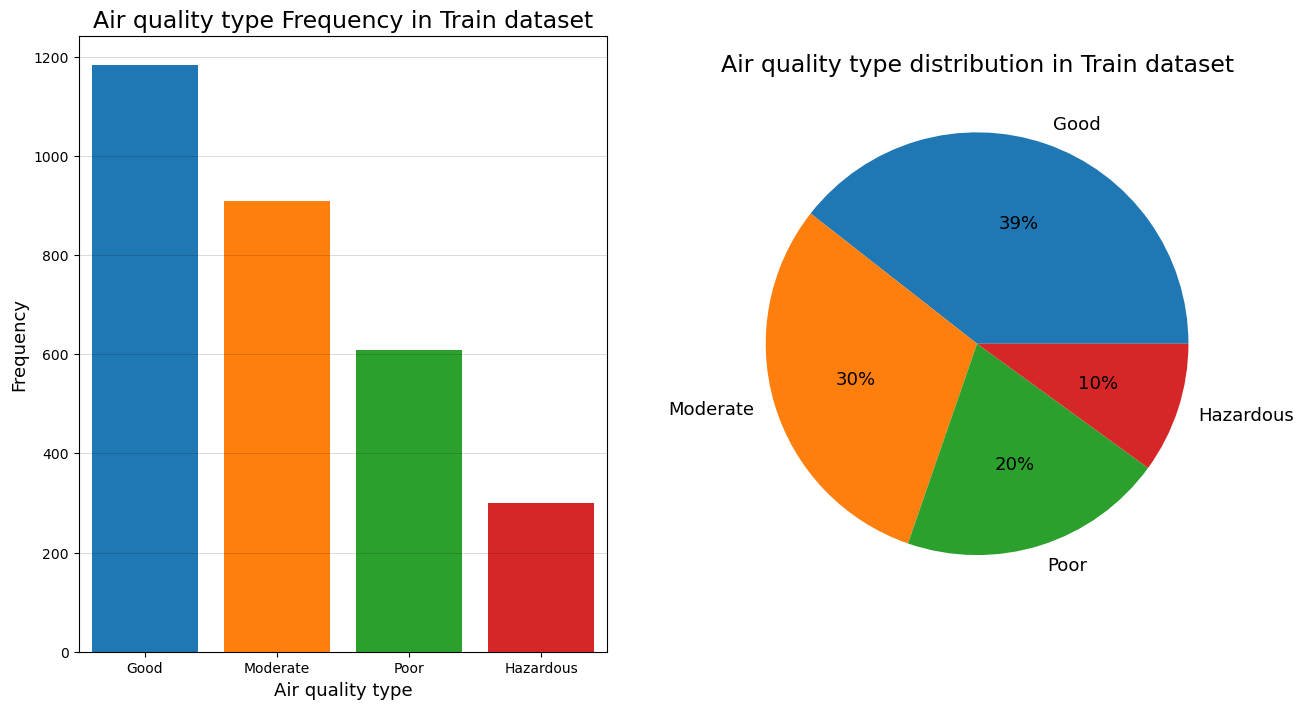
\includegraphics[keepaspectratio]{main_files/figure-pdf/cell-6-output-2.png}}

\begin{Shaded}
\begin{Highlighting}[]
\NormalTok{df\_original.info()}
\end{Highlighting}
\end{Shaded}

\begin{verbatim}
<class 'pandas.core.frame.DataFrame'>
Index: 3000 entries, 4576 to 860
Data columns (total 9 columns):
 #   Column                         Non-Null Count  Dtype  
---  ------                         --------------  -----  
 0   Temperature                    3000 non-null   float64
 1   Humidity                       3000 non-null   float64
 2   PM2.5                          3000 non-null   float64
 3   PM10                           3000 non-null   float64
 4   NO2                            3000 non-null   float64
 5   SO2                            3000 non-null   float64
 6   CO                             3000 non-null   float64
 7   Proximity_to_Industrial_Areas  3000 non-null   float64
 8   Population_Density             3000 non-null   int64  
dtypes: float64(8), int64(1)
memory usage: 234.4 KB
\end{verbatim}

\begin{Shaded}
\begin{Highlighting}[]
\NormalTok{fig, axes }\OperatorTok{=}\NormalTok{ plt.subplots(}\DecValTok{2}\NormalTok{, }\DecValTok{2}\NormalTok{, figsize}\OperatorTok{=}\NormalTok{(}\DecValTok{15}\NormalTok{, }\DecValTok{15}\NormalTok{))}

\NormalTok{ax }\OperatorTok{=}\NormalTok{ axes[}\DecValTok{0}\NormalTok{,}\DecValTok{0}\NormalTok{]}

\CommentTok{\# Plot the histogram}
\NormalTok{counts, bins, patches }\OperatorTok{=}\NormalTok{ ax.hist(df\_original[}\StringTok{"Temperature"}\NormalTok{], edgecolor}\OperatorTok{=}\StringTok{"black"}\NormalTok{, color}\OperatorTok{=}\StringTok{"skyblue"}\NormalTok{)}

\NormalTok{ax.set\_xticks(bins) }
\NormalTok{ax.set\_xticklabels([}\BuiltInTok{round}\NormalTok{(x) }\ControlFlowTok{for}\NormalTok{ x }\KeywordTok{in}\NormalTok{ bins])}

\CommentTok{\# Set titles and labels}
\NormalTok{ax.set\_title(}\StringTok{"Temperature histogram (Train)"}\NormalTok{, fontsize }\OperatorTok{=} \DecValTok{17}\NormalTok{)}
\NormalTok{ax.set\_xlabel(}\StringTok{"Temperature (°C)"}\NormalTok{, fontsize }\OperatorTok{=} \DecValTok{13}\NormalTok{)}
\NormalTok{ax.set\_ylabel(}\StringTok{"Frequency"}\NormalTok{, fontsize }\OperatorTok{=} \DecValTok{13}\NormalTok{)}

\ControlFlowTok{for}\NormalTok{ i, count }\KeywordTok{in} \BuiltInTok{enumerate}\NormalTok{(counts):}
\NormalTok{    ax.text(bins[i]}\OperatorTok{+}\FloatTok{2.5}\NormalTok{, count }\OperatorTok{+} \DecValTok{10}\NormalTok{, }\BuiltInTok{int}\NormalTok{(count), ha}\OperatorTok{=}\StringTok{"center"}\NormalTok{, va}\OperatorTok{=}\StringTok{"bottom"}\NormalTok{)}

\NormalTok{ax }\OperatorTok{=}\NormalTok{ axes[}\DecValTok{0}\NormalTok{,}\DecValTok{1}\NormalTok{]}

\CommentTok{\# Plot the histogram}
\NormalTok{counts, bins, patches }\OperatorTok{=}\NormalTok{ ax.hist(df\_original[}\StringTok{"Humidity"}\NormalTok{], edgecolor}\OperatorTok{=}\StringTok{"black"}\NormalTok{, color}\OperatorTok{=}\StringTok{"skyblue"}\NormalTok{)}

\NormalTok{ax.set\_xticks(bins) }
\NormalTok{ax.set\_xticklabels([}\BuiltInTok{int}\NormalTok{(x) }\ControlFlowTok{for}\NormalTok{ x }\KeywordTok{in}\NormalTok{ bins])}

\CommentTok{\# Set titles and labels}
\NormalTok{ax.set\_title(}\StringTok{"Humidity histogram (Train)"}\NormalTok{, fontsize }\OperatorTok{=} \DecValTok{17}\NormalTok{)}
\NormalTok{ax.set\_xlabel(}\StringTok{"Humidity (\%)"}\NormalTok{, fontsize }\OperatorTok{=} \DecValTok{13}\NormalTok{)}
\NormalTok{ax.set\_ylabel(}\StringTok{"Frequency"}\NormalTok{, fontsize }\OperatorTok{=} \DecValTok{13}\NormalTok{)}

\ControlFlowTok{for}\NormalTok{ i, count }\KeywordTok{in} \BuiltInTok{enumerate}\NormalTok{(counts):}
\NormalTok{    ax.text(bins[i]}\OperatorTok{+}\FloatTok{4.5}\NormalTok{, count }\OperatorTok{+} \DecValTok{10}\NormalTok{, }\BuiltInTok{int}\NormalTok{(count), ha}\OperatorTok{=}\StringTok{"center"}\NormalTok{, va}\OperatorTok{=}\StringTok{"bottom"}\NormalTok{)}


\NormalTok{ax }\OperatorTok{=}\NormalTok{ axes[}\DecValTok{1}\NormalTok{,}\DecValTok{0}\NormalTok{]}

\CommentTok{\# Plot the histogram}
\NormalTok{counts, bins, patches }\OperatorTok{=}\NormalTok{ ax.hist(df\_original[}\StringTok{"PM2.5"}\NormalTok{], edgecolor}\OperatorTok{=}\StringTok{"black"}\NormalTok{, color}\OperatorTok{=}\StringTok{"skyblue"}\NormalTok{)}

\NormalTok{ax.set\_xticks(bins)  }
\NormalTok{ax.set\_xticklabels([}\BuiltInTok{int}\NormalTok{(x) }\ControlFlowTok{for}\NormalTok{ x }\KeywordTok{in}\NormalTok{ bins])}

\CommentTok{\# Set titles and labels}
\NormalTok{ax.set\_title(}\StringTok{"PM2.5 histogram (Train)"}\NormalTok{, fontsize }\OperatorTok{=} \DecValTok{17}\NormalTok{)}
\NormalTok{ax.set\_xlabel(}\StringTok{"PM2.5 (µg/m³)"}\NormalTok{, fontsize }\OperatorTok{=} \DecValTok{13}\NormalTok{)}
\NormalTok{ax.set\_ylabel(}\StringTok{"Frequency"}\NormalTok{, fontsize }\OperatorTok{=} \DecValTok{13}\NormalTok{)}

\ControlFlowTok{for}\NormalTok{ i, count }\KeywordTok{in} \BuiltInTok{enumerate}\NormalTok{(counts):}
\NormalTok{    ax.text(bins[i]}\OperatorTok{+}\FloatTok{15.5}\NormalTok{, count }\OperatorTok{+} \DecValTok{10}\NormalTok{, }\BuiltInTok{int}\NormalTok{(count), ha}\OperatorTok{=}\StringTok{"center"}\NormalTok{, va}\OperatorTok{=}\StringTok{"bottom"}\NormalTok{)}

\NormalTok{ax }\OperatorTok{=}\NormalTok{ axes[}\DecValTok{1}\NormalTok{,}\DecValTok{1}\NormalTok{]}

\CommentTok{\# Plot the histogram}
\NormalTok{counts, bins, patches }\OperatorTok{=}\NormalTok{ ax.hist(df\_original[}\StringTok{"PM10"}\NormalTok{], edgecolor}\OperatorTok{=}\StringTok{"black"}\NormalTok{, color}\OperatorTok{=}\StringTok{"skyblue"}\NormalTok{)}

\NormalTok{ax.set\_xticks(bins) }
\NormalTok{ax.set\_xticklabels([}\BuiltInTok{int}\NormalTok{(x) }\ControlFlowTok{for}\NormalTok{ x }\KeywordTok{in}\NormalTok{ bins])}

\CommentTok{\# Set titles and labels}
\NormalTok{ax.set\_title(}\StringTok{"PM10 histogram (Train)"}\NormalTok{, fontsize }\OperatorTok{=} \DecValTok{17}\NormalTok{)}
\NormalTok{ax.set\_xlabel(}\StringTok{"PM10 (µg/m³)"}\NormalTok{, fontsize }\OperatorTok{=} \DecValTok{13}\NormalTok{)}
\NormalTok{ax.set\_ylabel(}\StringTok{"Frequency"}\NormalTok{, fontsize }\OperatorTok{=} \DecValTok{13}\NormalTok{)}

\ControlFlowTok{for}\NormalTok{ i, count }\KeywordTok{in} \BuiltInTok{enumerate}\NormalTok{(counts):}
\NormalTok{    ax.text(bins[i]}\OperatorTok{+}\FloatTok{15.5}\NormalTok{, count }\OperatorTok{+} \DecValTok{10}\NormalTok{, }\BuiltInTok{int}\NormalTok{(count), ha}\OperatorTok{=}\StringTok{"center"}\NormalTok{, va}\OperatorTok{=}\StringTok{"bottom"}\NormalTok{)}
\end{Highlighting}
\end{Shaded}

\pandocbounded{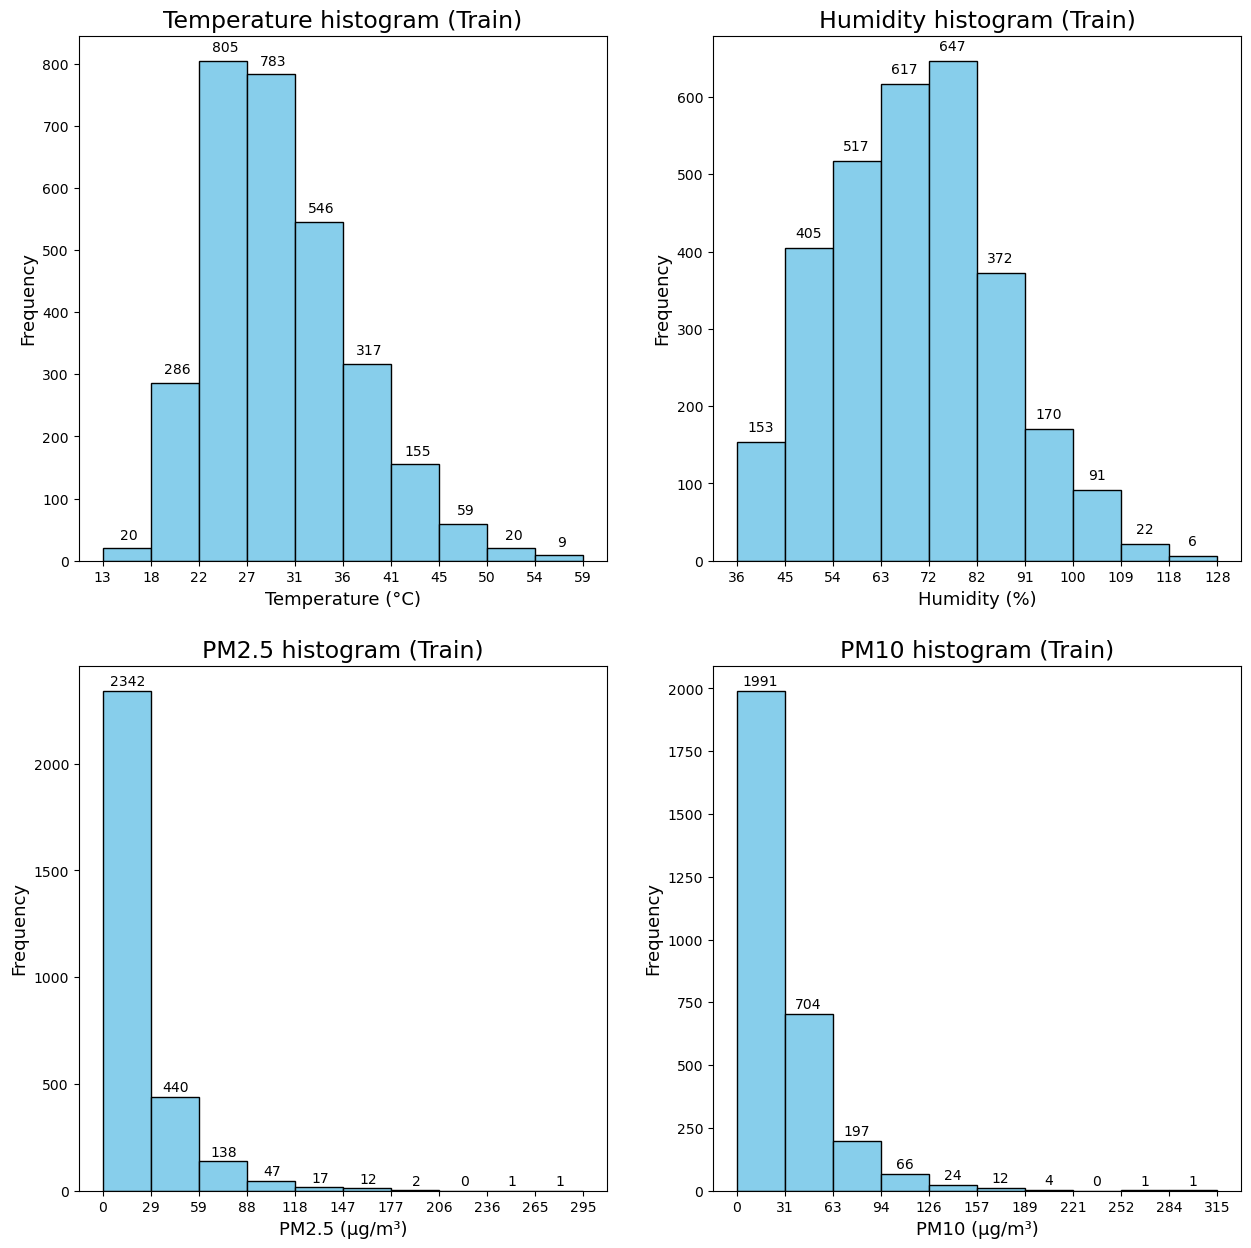
\includegraphics[keepaspectratio]{main_files/figure-pdf/cell-8-output-1.png}}

\begin{Shaded}
\begin{Highlighting}[]
\NormalTok{fig, axes }\OperatorTok{=}\NormalTok{ plt.subplots(}\DecValTok{2}\NormalTok{, }\DecValTok{2}\NormalTok{, figsize}\OperatorTok{=}\NormalTok{(}\DecValTok{15}\NormalTok{, }\DecValTok{15}\NormalTok{))}

\NormalTok{ax }\OperatorTok{=}\NormalTok{ axes[}\DecValTok{0}\NormalTok{,}\DecValTok{0}\NormalTok{]}

\CommentTok{\# Plot the histogram}
\NormalTok{counts, bins, patches }\OperatorTok{=}\NormalTok{ ax.hist(df\_original[}\StringTok{"NO2"}\NormalTok{], edgecolor}\OperatorTok{=}\StringTok{"black"}\NormalTok{, color}\OperatorTok{=}\StringTok{"skyblue"}\NormalTok{)}

\NormalTok{ax.set\_xticks(bins) }
\NormalTok{ax.set\_xticklabels([}\BuiltInTok{int}\NormalTok{(x) }\ControlFlowTok{for}\NormalTok{ x }\KeywordTok{in}\NormalTok{ bins])}

\CommentTok{\# Set titles and labels}
\NormalTok{ax.set\_title(}\StringTok{"NO2 histogram (Train)"}\NormalTok{, fontsize }\OperatorTok{=} \DecValTok{17}\NormalTok{)}
\NormalTok{ax.set\_xlabel(}\StringTok{"NO2 (ppb)"}\NormalTok{, fontsize }\OperatorTok{=} \DecValTok{13}\NormalTok{)}
\NormalTok{ax.set\_ylabel(}\StringTok{"Frequency"}\NormalTok{, fontsize }\OperatorTok{=} \DecValTok{13}\NormalTok{)}

\ControlFlowTok{for}\NormalTok{ i, count }\KeywordTok{in} \BuiltInTok{enumerate}\NormalTok{(counts):}
\NormalTok{    ax.text(bins[i]}\OperatorTok{+}\FloatTok{2.5}\NormalTok{, count }\OperatorTok{+} \DecValTok{10}\NormalTok{, }\BuiltInTok{int}\NormalTok{(count), ha}\OperatorTok{=}\StringTok{"center"}\NormalTok{, va}\OperatorTok{=}\StringTok{"bottom"}\NormalTok{)}

\NormalTok{ax }\OperatorTok{=}\NormalTok{ axes[}\DecValTok{0}\NormalTok{,}\DecValTok{1}\NormalTok{]}

\CommentTok{\# Plot the histogram}
\NormalTok{counts, bins, patches }\OperatorTok{=}\NormalTok{ ax.hist(df\_original[}\StringTok{"SO2"}\NormalTok{], edgecolor}\OperatorTok{=}\StringTok{"black"}\NormalTok{, color}\OperatorTok{=}\StringTok{"skyblue"}\NormalTok{)}

\NormalTok{ax.set\_xticks(bins) }
\NormalTok{ax.set\_xticklabels([}\BuiltInTok{int}\NormalTok{(x) }\ControlFlowTok{for}\NormalTok{ x }\KeywordTok{in}\NormalTok{ bins])}

\CommentTok{\# Set titles and labels}
\NormalTok{ax.set\_title(}\StringTok{"SO2 histogram (Train)"}\NormalTok{, fontsize }\OperatorTok{=} \DecValTok{17}\NormalTok{)}
\NormalTok{ax.set\_xlabel(}\StringTok{"SO2 (ppb)"}\NormalTok{, fontsize }\OperatorTok{=} \DecValTok{13}\NormalTok{)}
\NormalTok{ax.set\_ylabel(}\StringTok{"Frequency"}\NormalTok{, fontsize }\OperatorTok{=} \DecValTok{13}\NormalTok{)}

\ControlFlowTok{for}\NormalTok{ i, count }\KeywordTok{in} \BuiltInTok{enumerate}\NormalTok{(counts):}
\NormalTok{    ax.text(bins[i]}\OperatorTok{+}\FloatTok{2.5}\NormalTok{, count }\OperatorTok{+} \DecValTok{10}\NormalTok{, }\BuiltInTok{int}\NormalTok{(count), ha}\OperatorTok{=}\StringTok{"center"}\NormalTok{, va}\OperatorTok{=}\StringTok{"bottom"}\NormalTok{)}


\NormalTok{ax }\OperatorTok{=}\NormalTok{ axes[}\DecValTok{1}\NormalTok{,}\DecValTok{0}\NormalTok{]}

\CommentTok{\# Plot the histogram}
\NormalTok{counts, bins, patches }\OperatorTok{=}\NormalTok{ ax.hist(df\_original[}\StringTok{"CO"}\NormalTok{], edgecolor}\OperatorTok{=}\StringTok{"black"}\NormalTok{, color}\OperatorTok{=}\StringTok{"skyblue"}\NormalTok{)}

\NormalTok{ax.set\_xticks(bins)  }
\NormalTok{ax.set\_xticklabels([}\SpecialStringTok{f\textquotesingle{}}\SpecialCharTok{\{}\NormalTok{x}\SpecialCharTok{:.1f\}}\SpecialStringTok{\textquotesingle{}} \ControlFlowTok{for}\NormalTok{ x }\KeywordTok{in}\NormalTok{ bins]) }

\CommentTok{\# Set titles and labels}
\NormalTok{ax.set\_title(}\StringTok{"CO histogram (Train)"}\NormalTok{, fontsize }\OperatorTok{=} \DecValTok{17}\NormalTok{)}
\NormalTok{ax.set\_xlabel(}\StringTok{"CO (ppm)"}\NormalTok{, fontsize }\OperatorTok{=} \DecValTok{13}\NormalTok{)}
\NormalTok{ax.set\_ylabel(}\StringTok{"Frequency"}\NormalTok{, fontsize }\OperatorTok{=} \DecValTok{13}\NormalTok{)}

\ControlFlowTok{for}\NormalTok{ i, count }\KeywordTok{in} \BuiltInTok{enumerate}\NormalTok{(counts):}
\NormalTok{    ax.text(bins[i] }\OperatorTok{+} \FloatTok{0.15}\NormalTok{, count }\OperatorTok{+} \DecValTok{10}\NormalTok{, }\BuiltInTok{int}\NormalTok{(count), ha}\OperatorTok{=}\StringTok{"center"}\NormalTok{, va}\OperatorTok{=}\StringTok{"bottom"}\NormalTok{)}

\NormalTok{ax }\OperatorTok{=}\NormalTok{ axes[}\DecValTok{1}\NormalTok{,}\DecValTok{1}\NormalTok{]}

\CommentTok{\# Plot the histogram}
\NormalTok{counts, bins, patches }\OperatorTok{=}\NormalTok{ ax.hist(df\_original[}\StringTok{"Proximity\_to\_Industrial\_Areas"}\NormalTok{], edgecolor}\OperatorTok{=}\StringTok{"black"}\NormalTok{, color}\OperatorTok{=}\StringTok{"skyblue"}\NormalTok{)}

\NormalTok{ax.set\_xticks(bins) }
\NormalTok{ax.set\_xticklabels([}\BuiltInTok{int}\NormalTok{(x) }\ControlFlowTok{for}\NormalTok{ x }\KeywordTok{in}\NormalTok{ bins])}



\CommentTok{\# Set titles and labels}
\NormalTok{ax.set\_title(}\StringTok{"Proximity to Industrial Areas histogram (Train)"}\NormalTok{, fontsize }\OperatorTok{=} \DecValTok{17}\NormalTok{)}
\NormalTok{ax.set\_xlabel(}\StringTok{"Proximity to Industrial Areas (km)"}\NormalTok{, fontsize }\OperatorTok{=} \DecValTok{13}\NormalTok{)}
\NormalTok{ax.set\_ylabel(}\StringTok{"Frequency"}\NormalTok{, fontsize }\OperatorTok{=} \DecValTok{13}\NormalTok{)}

\ControlFlowTok{for}\NormalTok{ i, count }\KeywordTok{in} \BuiltInTok{enumerate}\NormalTok{(counts):}
\NormalTok{    ax.text(bins[i] }\OperatorTok{+}\NormalTok{ (bins[i}\OperatorTok{+}\DecValTok{1}\NormalTok{] }\OperatorTok{{-}}\NormalTok{ bins[i])}\OperatorTok{/}\DecValTok{2}\NormalTok{, count }\OperatorTok{+} \DecValTok{10}\NormalTok{, }\BuiltInTok{int}\NormalTok{(count), }
\NormalTok{            ha}\OperatorTok{=}\StringTok{"center"}\NormalTok{, va}\OperatorTok{=}\StringTok{"bottom"}\NormalTok{)}
\end{Highlighting}
\end{Shaded}

\pandocbounded{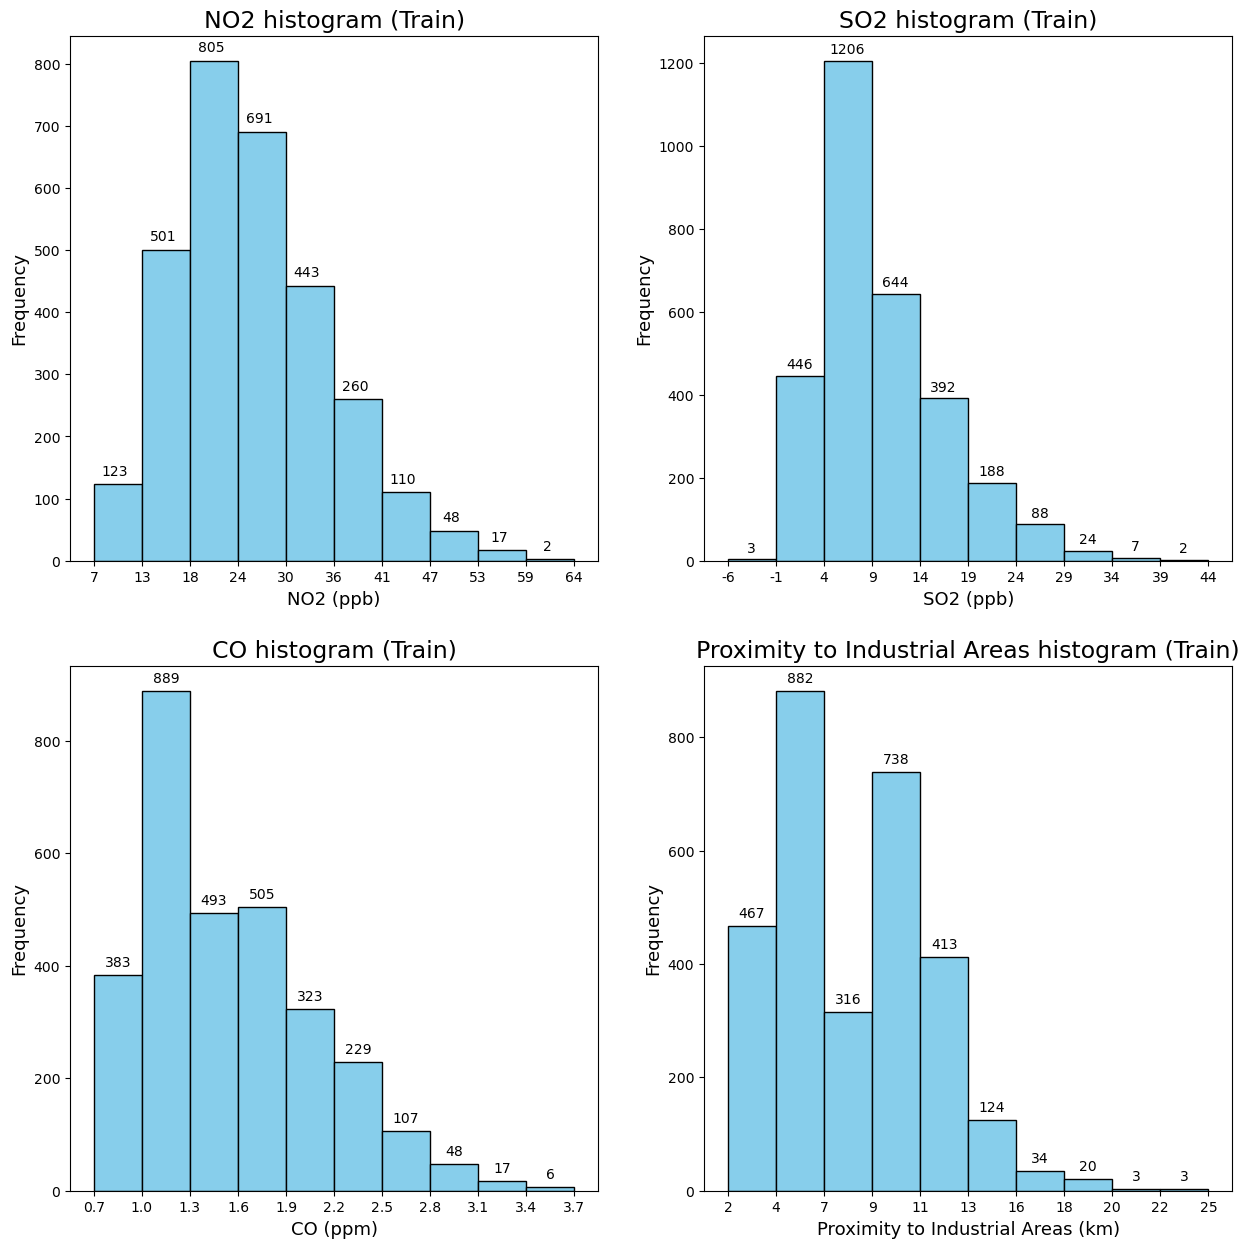
\includegraphics[keepaspectratio]{main_files/figure-pdf/cell-9-output-1.png}}

\begin{Shaded}
\begin{Highlighting}[]
\NormalTok{fig, axes }\OperatorTok{=}\NormalTok{ plt.subplots(}\DecValTok{2}\NormalTok{, }\DecValTok{2}\NormalTok{, figsize}\OperatorTok{=}\NormalTok{(}\DecValTok{13}\NormalTok{, }\DecValTok{13}\NormalTok{))}

\NormalTok{ax }\OperatorTok{=}\NormalTok{ axes[}\DecValTok{0}\NormalTok{,}\DecValTok{0}\NormalTok{]}
\CommentTok{\# Plot the histogram}
\NormalTok{counts, bins, patches }\OperatorTok{=}\NormalTok{ ax.hist(df\_original[}\StringTok{"Population\_Density"}\NormalTok{], edgecolor}\OperatorTok{=}\StringTok{"black"}\NormalTok{, color}\OperatorTok{=}\StringTok{"skyblue"}\NormalTok{)}

\NormalTok{ax.set\_xticks(bins) }
\NormalTok{ax.set\_xticklabels([}\BuiltInTok{int}\NormalTok{(x) }\ControlFlowTok{for}\NormalTok{ x }\KeywordTok{in}\NormalTok{ bins])}

\CommentTok{\# Set titles and labels}
\NormalTok{ax.set\_title(}\StringTok{"Population Density histogram (Train)"}\NormalTok{, fontsize }\OperatorTok{=} \DecValTok{17}\NormalTok{)}
\NormalTok{ax.set\_xlabel(}\StringTok{"Population Density (people/km²)"}\NormalTok{, fontsize }\OperatorTok{=} \DecValTok{13}\NormalTok{)}
\NormalTok{ax.set\_ylabel(}\StringTok{"Frequency"}\NormalTok{, fontsize }\OperatorTok{=} \DecValTok{13}\NormalTok{)}

\ControlFlowTok{for}\NormalTok{ i, count }\KeywordTok{in} \BuiltInTok{enumerate}\NormalTok{(counts):}
\NormalTok{    ax.text(bins[i]}\OperatorTok{+}\FloatTok{28.5}\NormalTok{, count }\OperatorTok{+} \DecValTok{5}\NormalTok{, }\BuiltInTok{int}\NormalTok{(count), ha}\OperatorTok{=}\StringTok{"center"}\NormalTok{, va}\OperatorTok{=}\StringTok{"bottom"}\NormalTok{)}

\NormalTok{axes[}\DecValTok{0}\NormalTok{,}\DecValTok{1}\NormalTok{].set\_visible(}\VariableTok{False}\NormalTok{)}
\NormalTok{axes[}\DecValTok{1}\NormalTok{,}\DecValTok{1}\NormalTok{].set\_visible(}\VariableTok{False}\NormalTok{)}
\NormalTok{axes[}\DecValTok{1}\NormalTok{,}\DecValTok{0}\NormalTok{].set\_visible(}\VariableTok{False}\NormalTok{)}
\end{Highlighting}
\end{Shaded}

\pandocbounded{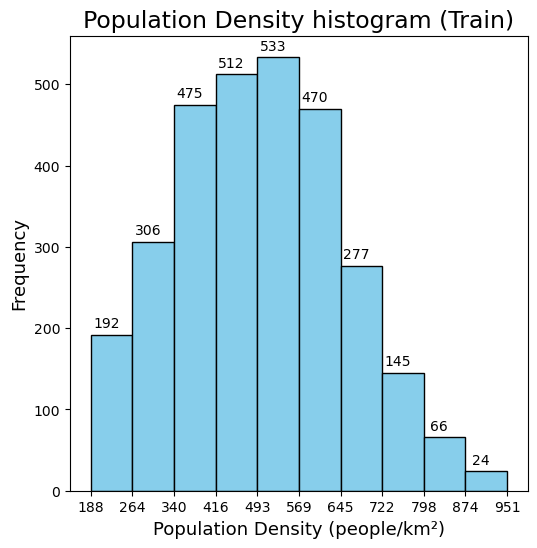
\includegraphics[keepaspectratio]{main_files/figure-pdf/cell-10-output-1.png}}

\section{Training the model}\label{training-the-model}

\[ \text{We are trying to solve supervised learning problem, where based on *p* features} X_{1}, ..., X_{p}\]
(\textbf{Temperature}, \textbf{Humidity}, \ldots) we want to predict the
value of target variable \(Y\) (\textbf{Air Quality}). We can put all of
these features into vector \(\textbf{X} = (X_{1}, ... X{_p})^T\) which
we will interpret as a random vector, and one of its specific
realization will be denoted as \(\mathbf{x}\). Let \(\mathcal{X}\) where
\(\textbf{x} \in \mathcal{X}\) be set containing all possible values of
these features, typically, and in our case,
\(\mathcal{X} = \mathbb{R}^p\). Then we can can describe our training
dataset as \textbf{N} pairs
\((\textbf{x}_{1}, Y_{1}), ..., (\textbf{x}_{N}, Y_{N})\) where
\(\textbf{x}_{i}\) is vector of features and \(Y_{i}\) is target
variable. The basic concept of predicting value of data point
\(\mathbf{x} \in \mathcal{X}\) is finding the k-closest points from it
(these points come from the train dataset). If we are solving regression
problems, we then take the average from the target varibles of the
k-closest neighbours. In classification problems (that's our case) we
take the most frequent value from the target variables of the k-closest
neighbours.\\
\strut \\
When trying to find the best model, there are many things to consider.
First of all we should define distance function.\\
\textbf{Distance} also called \textbf{metric} defined on set
\(\mathcal{X}\) is function d:
\(\mathcal{X} \times \mathcal{X} \rightarrow [0, +\infty)\) such that
for all \(x, y, z \in \mathcal{X}\), the following conditions holds:\\
\strut \\
\$ i);d(x,y) \geq 0\$, and \(d(x,y) = 0\) if and only if \(x = y\)
(positive definiteness)\\
\$ ii);d(x,y) = d(y,x)\$ (symmetry)\\
\$ iii);d(x,y) \geq d(x,z) + d(z,y)\$ (triangle inequalitext\{The most
common distance function used is KNN is Minkowski distance also called
q-norm defined as follows:\}\(\
\)\textbar\textbar x-y\textbar\textbar{}\emph{\{q\} = d}\{q\}(x,y) =
\sqrt[q]{\sum_{i=1}^{p} (x_i - y_i)^q}\$

After we have found k-nearest neighbours, we need to somehow decide what
value we should predict. In our case, we could just precict the value
with the most frequent target variable. What we can also do is try
weighted voting, that means that closer neighbours will have vote with
higher value.\\
Common choice for weight is inverse distance weighting\\
\(w_{i} = \frac{1}{d(x,y)}\)\\
For each category \(c\) that target variable can be, we count the total
weighted vote
\(W_{c} = \sum_{Y_i \in \mathcal{N}} w_i \cdot 1(Y_i = c)\)\\
where \(\mathcal{N}\) is set of target variables of k-nearest
neighbours. We then choose \$\hat{y} = \arg\max\_c W\_c \$, where \(c\)
is every possible category of target variable, as our prediction.

\section{Training the model}\label{training-the-model-1}

l We are trying to solve supervised learning problem, where based on
\emph{p} feature\$\$ X\_\{1\}, \ldots, X\_\{p\}\$ (\textbf{Temperature},
\textbf{Humidity}, \ldots) we want to predict the value of target
variable \(Y\) (\textbf{Air Quality}). We can put all of these features
into vector \(\textbf{X} = (X_{1}, ... X{_p})^T\) which we will
interpret as a random vector, and one of its specific realization will
be denoted as \(\mathbf{x}\). Let \(\mathcal{X}\) where
\(\textbf{x} \in \mathcal{X}\) be set containing all possible values of
these features, typically, and in our case,
\(\mathcal{X} = \mathbb{R}^p\). Then we can can describe our training
dataset as \textbf{N} pairs
\((\textbf{x}_{1}, Y_{1}), ..., (\textbf{x}_{N}, Y_{N})\) where
\(\textbf{x}_{i}\) is vector of features and \(Y_{i}\) is target
variable. The basic concept of predicting value of data point
\(\mathbf{x} \in \mathcal{X}\) is finding the k-closest points from it
(these points come from the train dataset). If we are solving regression
problems, we then take the average from the target varibles of the
k-closest neighbours. In classification problems (that's our case) we
take the most frequent value from the target variables of the k-closest
neighbours.\\
\strut \\
When trying to find the best model, there are many things to consider.
First of all we should define distance function.\\
\textbf{Distance} also called \textbf{metric} defined on set
\(\mathcal{X}\) is function d:
\(\mathcal{X} \times \mathcal{X} \rightarrow [0, +\infty)\) such that
for all \(x, y, z \in \mathcal{X}\), the following conditions holds:\\
\$ i);d(x,y) \geq 0\$, and \(d(x,y) = 0\) if and only if \(x = y\)
(positive definiteness)\\
\$ ii);d(x,y) = d(y,x)\$ (symmetry)\\
\$ iii);d(x,y) \geq d(x,z) + d(z,y)\$ (triangle inequality)

\(\text{The most common distance function used is KNN is Minkowski distance also called q-norm defined as follows:}\)\\
\(||x-y||_{q} = d_{q}(x,y) = \sqrt[q]{\sum_{i=1}^{p} (x_i - y_i)^q}\)

After we have found k-nearest neighbours, we need to somehow decide what
value we should predict. In our case, we could just precict the value
with the most frequent target variable. What we can also do is try
weighted voting, that means that closer neighbours will have vote with
higher value.\\
Common choice for weight is inverse distance weighting\\
\(w_{i} = \frac{1}{d(x,y)}\)\\
For each category \(c\) that target variable can be, we count the total
weighted vote
\(W_{c} = \sum_{Y_i \in \mathcal{N}} w_i \cdot 1(Y_i = c)\)\\
where \(\mathcal{N}\) is set of target variables of k-nearest
neighbours. We then choose \$\hat{y} = \arg\max\_c W\_c \$, where \(c\)
is every possible category of target variable, as our prediction.

\begin{Shaded}
\begin{Highlighting}[]
\KeywordTok{def}\NormalTok{ train\_model(}\OperatorTok{*}\NormalTok{args,}\OperatorTok{**}\NormalTok{kwargs):}
    \CommentTok{"""Function, that trains model with specific paraketrs, defined in kwargs.}
\CommentTok{    {-}{-}{-}}
\CommentTok{    Attributes:}
\CommentTok{    *args: Xtrain,Ytrain}
\CommentTok{    **kwargs: options for training model}
\CommentTok{    {-}{-}{-}}
\CommentTok{    Return: trained model}
\CommentTok{    """}
\NormalTok{    X }\OperatorTok{=}\NormalTok{ args[}\DecValTok{0}\NormalTok{]}
\NormalTok{    y }\OperatorTok{=}\NormalTok{ args[}\DecValTok{1}\NormalTok{]}
    \ControlFlowTok{return}\NormalTok{ KNeighborsClassifier(}\OperatorTok{**}\NormalTok{kwargs).fit(X,y)}
\end{Highlighting}
\end{Shaded}

\section{Finding the Best model (Hyperparameter
tuning)}\label{finding-the-best-model-hyperparameter-tuning}

When finding the best model, there are many things to consider. Our goal
is to somehow maximize the classification accuracy on new data, that the
model has never seen before. Accuracy is defined as\\
\(\frac{ \text{number of correctly classified}}{ \text{number of all classified}}\).
The accuracy which we are trying to maximize is the accuracy of how our
model built using \textbf{train} dataset will predict on
\textbf{validating} dataset. In order to maximize this accuracy, we can
try changing the number of neighbours (k), then we can try changing the
distance metric, lastly, we can try whether using weighted distance
makes any difference. We build our model using combination of these
different possibilites and for every one of them we meassure the
accuracy on \textbf{validating} dataset. We then choose the model with
the highest accuracy.

\begin{Shaded}
\begin{Highlighting}[]
\KeywordTok{def}\NormalTok{ find\_best(}\OperatorTok{*}\NormalTok{args):}
    \CommentTok{""" Function finding best parametrs for specified data}
\CommentTok{    {-}{-}{-}}
\CommentTok{    Attributes:}
\CommentTok{    Xtrain, ytrain, Xval, Yval}
\CommentTok{    """}
\NormalTok{    param\_grid }\OperatorTok{=}\NormalTok{ \{}
        \StringTok{\textquotesingle{}n\_neighbors\textquotesingle{}}\NormalTok{: }\BuiltInTok{range}\NormalTok{(}\DecValTok{1}\NormalTok{,}\DecValTok{15}\NormalTok{), }
        \StringTok{\textquotesingle{}p\textquotesingle{}}\NormalTok{: }\BuiltInTok{range}\NormalTok{(}\DecValTok{1}\NormalTok{,}\DecValTok{4}\NormalTok{),}
        \StringTok{\textquotesingle{}weights\textquotesingle{}}\NormalTok{: [}\StringTok{\textquotesingle{}uniform\textquotesingle{}}\NormalTok{, }\StringTok{\textquotesingle{}distance\textquotesingle{}}\NormalTok{]}
\NormalTok{    \}}
\NormalTok{    param\_comb }\OperatorTok{=}\NormalTok{ ParameterGrid(param\_grid)}
\NormalTok{    val\_acc }\OperatorTok{=}\NormalTok{ []}
\NormalTok{    train\_acc }\OperatorTok{=}\NormalTok{ []}
    \ControlFlowTok{for}\NormalTok{ params }\KeywordTok{in}\NormalTok{ param\_comb:}
\NormalTok{        clfKNN }\OperatorTok{=}\NormalTok{ KNeighborsClassifier(}\OperatorTok{**}\NormalTok{params)}
\NormalTok{        clfKNN.fit(args[}\DecValTok{0}\NormalTok{], args[}\DecValTok{1}\NormalTok{])}
\NormalTok{        train\_acc.append(clfKNN.score(args[}\DecValTok{0}\NormalTok{],args[}\DecValTok{1}\NormalTok{]))}
\NormalTok{        val\_acc.append(clfKNN.score(args[}\DecValTok{2}\NormalTok{],args[}\DecValTok{3}\NormalTok{]))}
    \ControlFlowTok{return}\NormalTok{ param\_comb[np.argmax(val\_acc)], train\_acc, val\_acc}
\end{Highlighting}
\end{Shaded}

\begin{Shaded}
\begin{Highlighting}[]
\NormalTok{best\_params\_no\_scale, train\_acc, val\_acc }\OperatorTok{=}\NormalTok{ find\_best(Xtrain,ytrain,Xval,yval)}

\NormalTok{scaler }\OperatorTok{=}\NormalTok{ StandardScaler()}
\NormalTok{Xtrain\_fit }\OperatorTok{=}\NormalTok{ scaler.fit\_transform(Xtrain)}
\NormalTok{Xval\_fit }\OperatorTok{=}\NormalTok{ scaler.transform(Xval)}
\NormalTok{best\_params\_standard, train\_acc\_standard, val\_acc\_standard }\OperatorTok{=}\NormalTok{ find\_best(Xtrain\_fit,ytrain,Xval\_fit,yval)}

\NormalTok{scaler }\OperatorTok{=}\NormalTok{ MinMaxScaler()}
\NormalTok{Xtrain\_fit }\OperatorTok{=}\NormalTok{ scaler.fit\_transform(Xtrain)}
\NormalTok{Xval\_fit }\OperatorTok{=}\NormalTok{ scaler.transform(Xval)}
\NormalTok{best\_params\_minmax, train\_acc\_minmax, val\_acc\_minmax }\OperatorTok{=}\NormalTok{ find\_best(Xtrain\_fit,ytrain,Xval\_fit,yval)}
\end{Highlighting}
\end{Shaded}

\subsection{No normalization accuracy}\label{no-normalization-accuracy}

Using no normalization, the best accuracy we get is 0.833

\begin{Shaded}
\begin{Highlighting}[]
\NormalTok{clfKNN }\OperatorTok{=}\NormalTok{ KNeighborsClassifier(}\OperatorTok{**}\NormalTok{best\_params\_no\_scale)}
\NormalTok{clfKNN.fit(Xtrain, ytrain)}
\NormalTok{y\_knn\_val }\OperatorTok{=}\NormalTok{ clfKNN.predict(Xval)}
\NormalTok{display(metrics.accuracy\_score(yval, y\_knn\_val))}
\end{Highlighting}
\end{Shaded}

\begin{verbatim}
0.833
\end{verbatim}

\begin{Shaded}
\begin{Highlighting}[]
\NormalTok{fig, ax }\OperatorTok{=}\NormalTok{ plt.subplots(figsize}\OperatorTok{=}\NormalTok{(}\DecValTok{15}\NormalTok{,}\DecValTok{5}\NormalTok{))}
\NormalTok{ax.set\_title(}\StringTok{"Model accuracy on Training and Validating datasets based on hyperparameter index (no normalization)"}\NormalTok{, fontsize}\OperatorTok{=}\DecValTok{17}\NormalTok{)}
\NormalTok{ax.plot(train\_acc,}\StringTok{\textquotesingle{}or{-}\textquotesingle{}}\NormalTok{)}
\NormalTok{ax.plot(val\_acc,}\StringTok{\textquotesingle{}ob{-}\textquotesingle{}}\NormalTok{)}


\NormalTok{max\_idx }\OperatorTok{=}\NormalTok{ np.argmax(val\_acc)}
\NormalTok{ax.plot(max\_idx, val\_acc[max\_idx], marker}\OperatorTok{=}\StringTok{\textquotesingle{}o\textquotesingle{}}\NormalTok{, color}\OperatorTok{=}\StringTok{\textquotesingle{}\#77DD77\textquotesingle{}}\NormalTok{, markersize}\OperatorTok{=}\DecValTok{13}\NormalTok{, markeredgecolor}\OperatorTok{=}\StringTok{\textquotesingle{}black\textquotesingle{}}\NormalTok{, markeredgewidth}\OperatorTok{=}\DecValTok{2}\NormalTok{)}
\NormalTok{ax.set\_ylim(bottom}\OperatorTok{=}\FloatTok{0.67}\NormalTok{, top}\OperatorTok{=}\FloatTok{1.02}\NormalTok{)}

\NormalTok{ax.set\_xlabel(}\StringTok{\textquotesingle{}Hyperparameter index\textquotesingle{}}\NormalTok{, fontsize}\OperatorTok{=}\DecValTok{13}\NormalTok{)}
\NormalTok{ax.set\_ylabel(}\StringTok{\textquotesingle{}Accuracy\textquotesingle{}}\NormalTok{, fontsize}\OperatorTok{=}\DecValTok{13}\NormalTok{)}
\NormalTok{ax.legend([}\StringTok{\textquotesingle{}Train\textquotesingle{}}\NormalTok{, }\StringTok{\textquotesingle{}Validate\textquotesingle{}}\NormalTok{, }\StringTok{\textquotesingle{}Best validate accuracy\textquotesingle{}}\NormalTok{], loc}\OperatorTok{=}\StringTok{\textquotesingle{}lower right\textquotesingle{}}\NormalTok{)}
\end{Highlighting}
\end{Shaded}

\pandocbounded{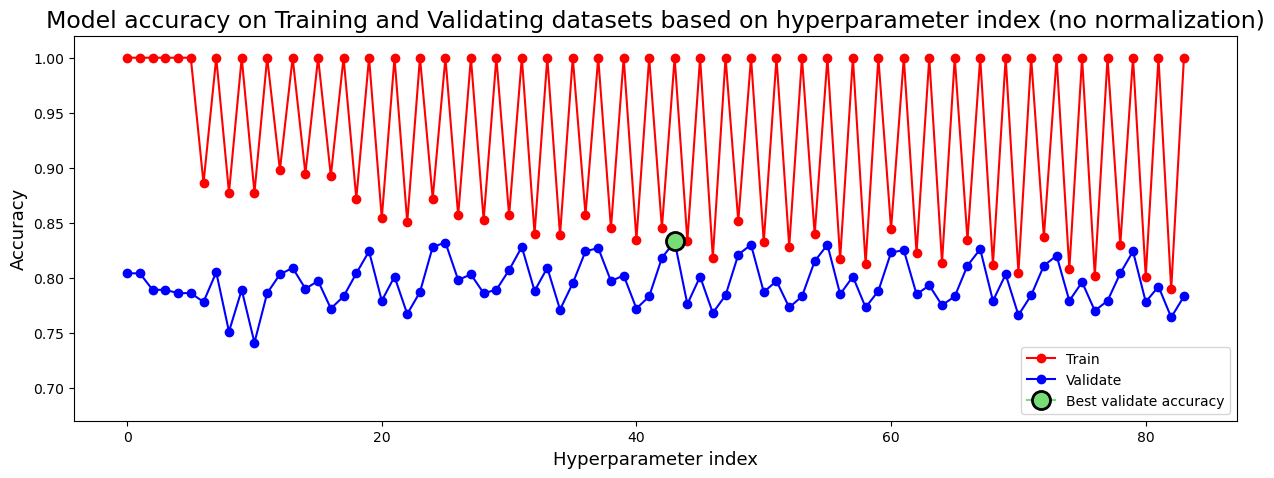
\includegraphics[keepaspectratio]{main_files/figure-pdf/cell-15-output-1.png}}

\section{Normalization}\label{normalization}

One technique that can also help with making the model more accurate is
normalization. In some cases, the features are difficult to compare and
it is essentially impossible to find a universal measure. This can be
addressed by using clever methods to normalize the data using linear
transformation. The simplest method used to normalize data is called
\textbf{Min-Max} normalization which scales every element in selected
feature into interval \([0,1]\). It is defined as follows:\\
For given feature let's call its minimal value \(\text{min}_x\) and the
maximal value \(\text{max}_x\), then we will define the value \(x_i\) of
this feature as\\
\(x_i \leftarrow \frac{ x_i - \text{min}_x}{ \text{max}_i - \text{min}_x}\)

Another commonly used normalization method is standardization, defined
as follows \(x_i \leftarrow \frac{x_i - \bar{x}}{\sqrt{s_x^2}}\) where
\(\bar{x} = \frac{1}{n} \sum_{i} x_i\) is sample mean and
\(s_x^2 = \frac{1}{n-1} \sum_{i}^{} {(x_i - \bar{x})^2}\) is sample
variance

\subsection{Standardization accuracy}\label{standardization-accuracy}

Using Standardization, the best accuracy we get is 0.931

\begin{Shaded}
\begin{Highlighting}[]
\NormalTok{scaler }\OperatorTok{=}\NormalTok{ StandardScaler()}
\NormalTok{Xtrain\_fit }\OperatorTok{=}\NormalTok{ scaler.fit\_transform(Xtrain)}
\NormalTok{Xval\_fit }\OperatorTok{=}\NormalTok{ scaler.transform(Xval)}

\NormalTok{clfKNN }\OperatorTok{=}\NormalTok{ KNeighborsClassifier(}\OperatorTok{**}\NormalTok{best\_params\_standard)}
\NormalTok{clfKNN.fit(Xtrain\_fit, ytrain)}
\NormalTok{y\_knn\_val }\OperatorTok{=}\NormalTok{ clfKNN.predict(Xval\_fit)}
\NormalTok{display(metrics.accuracy\_score(yval, y\_knn\_val))}
\end{Highlighting}
\end{Shaded}

\begin{verbatim}
0.931
\end{verbatim}

\begin{Shaded}
\begin{Highlighting}[]
\NormalTok{fig, ax }\OperatorTok{=}\NormalTok{ plt.subplots(figsize}\OperatorTok{=}\NormalTok{(}\DecValTok{15}\NormalTok{,}\DecValTok{5}\NormalTok{))}
\NormalTok{ax.set\_title(}\StringTok{"Model accuracy on Training and Validating datasets based on hyperparameter index (standardization)"}\NormalTok{, fontsize}\OperatorTok{=}\DecValTok{17}\NormalTok{)}
\NormalTok{ax.plot(train\_acc\_standard,}\StringTok{\textquotesingle{}or{-}\textquotesingle{}}\NormalTok{)}
\NormalTok{ax.plot(val\_acc\_standard,}\StringTok{\textquotesingle{}ob{-}\textquotesingle{}}\NormalTok{)}


\NormalTok{max\_idx }\OperatorTok{=}\NormalTok{ np.argmax(val\_acc\_standard)}
\CommentTok{\#display(val\_acc\_standard[max\_idx])}
\NormalTok{ax.plot(max\_idx, val\_acc\_standard[max\_idx], marker}\OperatorTok{=}\StringTok{\textquotesingle{}o\textquotesingle{}}\NormalTok{, color}\OperatorTok{=}\StringTok{\textquotesingle{}\#77DD77\textquotesingle{}}\NormalTok{, markersize}\OperatorTok{=}\DecValTok{13}\NormalTok{, markeredgecolor}\OperatorTok{=}\StringTok{\textquotesingle{}black\textquotesingle{}}\NormalTok{, markeredgewidth}\OperatorTok{=}\DecValTok{2}\NormalTok{)}

\NormalTok{ax.set\_xlabel(}\StringTok{\textquotesingle{}Hyperparameter index\textquotesingle{}}\NormalTok{, fontsize}\OperatorTok{=}\DecValTok{13}\NormalTok{)}
\NormalTok{ax.set\_ylabel(}\StringTok{\textquotesingle{}Accuracy\textquotesingle{}}\NormalTok{, fontsize}\OperatorTok{=}\DecValTok{13}\NormalTok{)}
\NormalTok{ax.legend([}\StringTok{\textquotesingle{}Train\textquotesingle{}}\NormalTok{, }\StringTok{\textquotesingle{}Validate\textquotesingle{}}\NormalTok{, }\StringTok{\textquotesingle{}Best validate accuracy\textquotesingle{}}\NormalTok{])}
\end{Highlighting}
\end{Shaded}

\pandocbounded{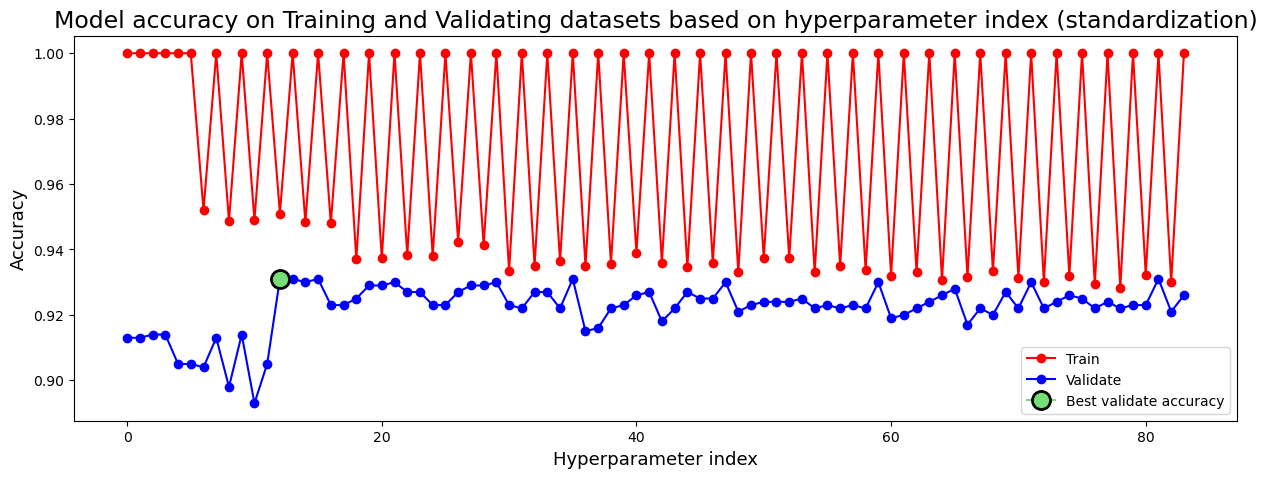
\includegraphics[keepaspectratio]{main_files/figure-pdf/cell-17-output-1.png}}

\subsection{Min-Max accuracy}\label{min-max-accuracy}

Using Min-Max normalization, the best accuracy we get is 0.942

\begin{Shaded}
\begin{Highlighting}[]
\NormalTok{scaler }\OperatorTok{=}\NormalTok{ MinMaxScaler()}
\NormalTok{Xtrain\_fit }\OperatorTok{=}\NormalTok{ scaler.fit\_transform(Xtrain)}
\NormalTok{Xval\_fit }\OperatorTok{=}\NormalTok{ scaler.transform(Xval)}

\NormalTok{clfKNN }\OperatorTok{=}\NormalTok{ KNeighborsClassifier(}\OperatorTok{**}\NormalTok{best\_params\_minmax)}
\NormalTok{clfKNN.fit(Xtrain\_fit, ytrain)}
\NormalTok{y\_knn\_val }\OperatorTok{=}\NormalTok{ clfKNN.predict(Xval\_fit)}
\NormalTok{display(metrics.accuracy\_score(yval, y\_knn\_val))}
\end{Highlighting}
\end{Shaded}

\begin{verbatim}
0.942
\end{verbatim}

\begin{Shaded}
\begin{Highlighting}[]
\NormalTok{fig, ax }\OperatorTok{=}\NormalTok{ plt.subplots(figsize}\OperatorTok{=}\NormalTok{(}\DecValTok{15}\NormalTok{,}\DecValTok{5}\NormalTok{))}
\NormalTok{ax.set\_title(}\StringTok{"Model accuracy on Training and Validating datasets based on hyperparameter index (min{-}max normalization)"}\NormalTok{, fontsize}\OperatorTok{=}\DecValTok{17}\NormalTok{)}
\NormalTok{ax.plot(train\_acc\_minmax,}\StringTok{\textquotesingle{}or{-}\textquotesingle{}}\NormalTok{)}
\NormalTok{ax.plot(val\_acc\_minmax,}\StringTok{\textquotesingle{}ob{-}\textquotesingle{}}\NormalTok{)}


\NormalTok{max\_idx }\OperatorTok{=}\NormalTok{ np.argmax(val\_acc\_minmax)}
\CommentTok{\#display(val\_acc\_minmax[max\_idx])}
\NormalTok{ax.plot(max\_idx, val\_acc\_minmax[max\_idx], marker}\OperatorTok{=}\StringTok{\textquotesingle{}o\textquotesingle{}}\NormalTok{, color}\OperatorTok{=}\StringTok{\textquotesingle{}\#77DD77\textquotesingle{}}\NormalTok{, markersize}\OperatorTok{=}\DecValTok{13}\NormalTok{, markeredgecolor}\OperatorTok{=}\StringTok{\textquotesingle{}black\textquotesingle{}}\NormalTok{, markeredgewidth}\OperatorTok{=}\DecValTok{2}\NormalTok{)}

\NormalTok{ax.set\_xlabel(}\StringTok{\textquotesingle{}Hyperparameter index\textquotesingle{}}\NormalTok{, fontsize}\OperatorTok{=}\DecValTok{13}\NormalTok{)}
\NormalTok{ax.set\_ylabel(}\StringTok{\textquotesingle{}Accuracy\textquotesingle{}}\NormalTok{, fontsize}\OperatorTok{=}\DecValTok{13}\NormalTok{)}
\NormalTok{ax.legend([}\StringTok{\textquotesingle{}Train\textquotesingle{}}\NormalTok{, }\StringTok{\textquotesingle{}Validate\textquotesingle{}}\NormalTok{, }\StringTok{\textquotesingle{}Best validate accuracy\textquotesingle{}}\NormalTok{])}
\end{Highlighting}
\end{Shaded}

\pandocbounded{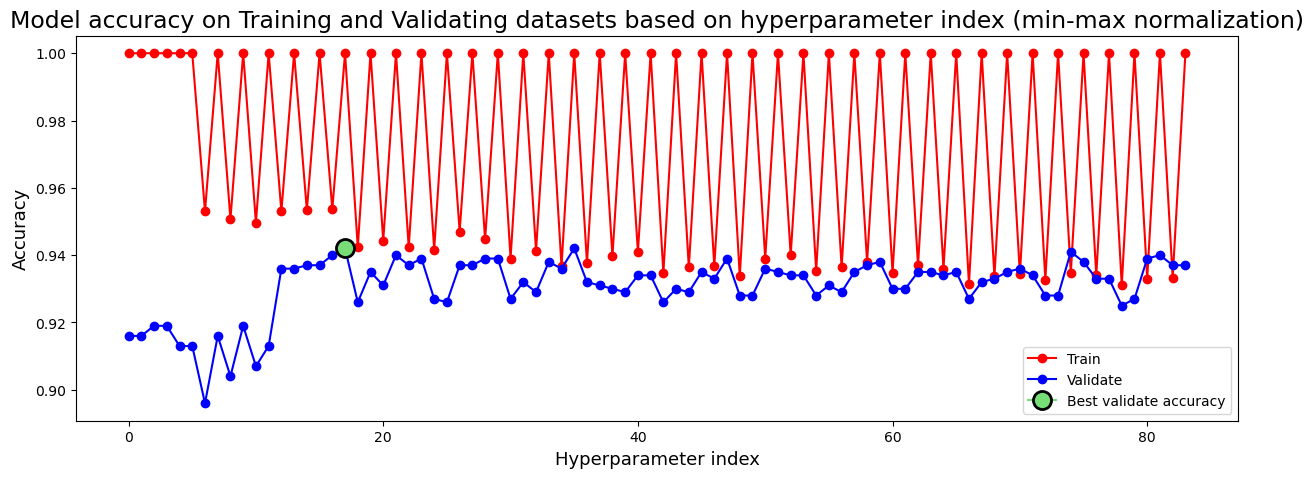
\includegraphics[keepaspectratio]{main_files/figure-pdf/cell-19-output-1.png}}

\section{Interactive graph}\label{interactive-graph}

Here we have an interactive graph that shows how our model predicts on
validating datasets based on different hyperparameters.

\begin{Shaded}
\begin{Highlighting}[]
\NormalTok{color\_map }\OperatorTok{=}\NormalTok{ \{}
    \StringTok{\textquotesingle{}Good\textquotesingle{}}\NormalTok{: }\StringTok{\textquotesingle{}green\textquotesingle{}}\NormalTok{,}
    \StringTok{\textquotesingle{}Moderate\textquotesingle{}}\NormalTok{: }\StringTok{\textquotesingle{}yellow\textquotesingle{}}\NormalTok{,}
    \StringTok{\textquotesingle{}Poor\textquotesingle{}}\NormalTok{: }\StringTok{\textquotesingle{}orange\textquotesingle{}}\NormalTok{,}
    \StringTok{\textquotesingle{}Hazardous\textquotesingle{}}\NormalTok{: }\StringTok{\textquotesingle{}red\textquotesingle{}}
\NormalTok{\}}
\NormalTok{category\_order }\OperatorTok{=}\NormalTok{ [}\StringTok{"Good"}\NormalTok{, }\StringTok{"Moderate"}\NormalTok{, }\StringTok{"Poor"}\NormalTok{, }\StringTok{"Hazardous"}\NormalTok{]}
\end{Highlighting}
\end{Shaded}

\begin{Shaded}
\begin{Highlighting}[]
\KeywordTok{def}\NormalTok{ show\_graph(X, y\_pred, x\_ax}\OperatorTok{=}\StringTok{\textquotesingle{}Proximity\_to\_Industrial\_Areas\textquotesingle{}}\NormalTok{, y\_ax}\OperatorTok{=}\StringTok{\textquotesingle{}CO\textquotesingle{}}\NormalTok{):}
\NormalTok{    df\_viz }\OperatorTok{=}\NormalTok{ X.copy()}
\NormalTok{    df\_viz[}\StringTok{\textquotesingle{}Air Quality\textquotesingle{}}\NormalTok{] }\OperatorTok{=}\NormalTok{ y\_pred}
\NormalTok{    fig }\OperatorTok{=}\NormalTok{ px.scatter(df\_viz, x}\OperatorTok{=}\NormalTok{x\_ax, y}\OperatorTok{=}\NormalTok{y\_ax, color}\OperatorTok{=}\StringTok{\textquotesingle{}Air Quality\textquotesingle{}}\NormalTok{, color\_discrete\_map}\OperatorTok{=}\NormalTok{color\_map,}
\NormalTok{                     hover\_data}\OperatorTok{=}\NormalTok{df\_viz, title}\OperatorTok{=}\StringTok{\textquotesingle{}KNN Visualization\textquotesingle{}}\NormalTok{,}
\NormalTok{                     category\_orders}\OperatorTok{=}\NormalTok{\{}\StringTok{\textquotesingle{}Air Quality\textquotesingle{}}\NormalTok{:category\_order\})}

\NormalTok{    fig.update\_layout(}
\NormalTok{        title\_font}\OperatorTok{=}\BuiltInTok{dict}\NormalTok{(size}\OperatorTok{=}\DecValTok{27}\NormalTok{), }
\NormalTok{        xaxis\_title\_font}\OperatorTok{=}\BuiltInTok{dict}\NormalTok{(size}\OperatorTok{=}\DecValTok{19}\NormalTok{), }
\NormalTok{        yaxis\_title\_font}\OperatorTok{=}\BuiltInTok{dict}\NormalTok{(size}\OperatorTok{=}\DecValTok{19}\NormalTok{),}
\NormalTok{        xaxis\_title}\OperatorTok{=}\StringTok{"Proximity to Industrial Areas (km)"}\NormalTok{,}
\NormalTok{        yaxis\_title}\OperatorTok{=}\StringTok{"CO (ppm)"}\NormalTok{,}
\NormalTok{        height }\OperatorTok{=} \DecValTok{550}
\NormalTok{    )}
    
\NormalTok{    fig.show()}
\end{Highlighting}
\end{Shaded}

\begin{Shaded}
\begin{Highlighting}[]
\NormalTok{n\_neighbors\_slider }\OperatorTok{=}\NormalTok{ widgets.IntSlider(value}\OperatorTok{=}\DecValTok{5}\NormalTok{, }\BuiltInTok{min}\OperatorTok{=}\DecValTok{1}\NormalTok{, }\BuiltInTok{max}\OperatorTok{=}\DecValTok{20}\NormalTok{, step}\OperatorTok{=}\DecValTok{1}\NormalTok{, description}\OperatorTok{=}\StringTok{"n\_neighbors"}\NormalTok{)}
\NormalTok{p\_slider }\OperatorTok{=}\NormalTok{ widgets.IntSlider(value}\OperatorTok{=}\DecValTok{5}\NormalTok{, }\BuiltInTok{min}\OperatorTok{=}\DecValTok{1}\NormalTok{, }\BuiltInTok{max}\OperatorTok{=}\DecValTok{20}\NormalTok{, step}\OperatorTok{=}\DecValTok{1}\NormalTok{, description}\OperatorTok{=}\StringTok{"p\_metric"}\NormalTok{)}
\NormalTok{scale }\OperatorTok{=}\NormalTok{ widgets.RadioButtons(}
\NormalTok{    options}\OperatorTok{=}\NormalTok{[}\StringTok{\textquotesingle{}None\textquotesingle{}}\NormalTok{, }\StringTok{\textquotesingle{}Standard\textquotesingle{}}\NormalTok{, }\StringTok{\textquotesingle{}MinMax\textquotesingle{}}\NormalTok{],}
\NormalTok{    description}\OperatorTok{=}\StringTok{\textquotesingle{}Choose normalization:\textquotesingle{}}\NormalTok{,}
\NormalTok{    disabled}\OperatorTok{=}\VariableTok{False}
\NormalTok{)}
\NormalTok{weights }\OperatorTok{=}\NormalTok{ widgets.RadioButtons(}
\NormalTok{    options}\OperatorTok{=}\NormalTok{[}\StringTok{\textquotesingle{}uniform\textquotesingle{}}\NormalTok{, }\StringTok{\textquotesingle{}distance\textquotesingle{}}\NormalTok{],}
\NormalTok{    description}\OperatorTok{=}\StringTok{\textquotesingle{}Chose weight:\textquotesingle{}}
\NormalTok{)}
\end{Highlighting}
\end{Shaded}

\phantomsection\label{dynamic_graph}
\begin{verbatim}
interactive(children=(IntSlider(value=5, description='n_neighbors', max=20, min=1), IntSlider(value=5, descrip…
\end{verbatim}

Interactive KNN visualization

\section{Choosing the final model}\label{choosing-the-final-model}

Based on the results, we can see that the best model is the model that
uses Min-Max normalization, uses weighted distance, 3-norm and 3
neighbours with accuracy of 0.942 We can graph confusion matrix, that
shows how accurately we predicted each type of category. Finally, we
will predict the expected accuracy on the \textbf{test} dataset, which
will give us an estimate of how accurately the model will perform on
new, unseen data.

\begin{Shaded}
\begin{Highlighting}[]
\NormalTok{best\_params\_minmax}
\end{Highlighting}
\end{Shaded}

\begin{verbatim}
{'weights': 'distance', 'p': 3, 'n_neighbors': 3}
\end{verbatim}

\begin{Shaded}
\begin{Highlighting}[]
\NormalTok{max\_idx }\OperatorTok{=}\NormalTok{ np.argmax(val\_acc)}
\NormalTok{max\_idx\_standard }\OperatorTok{=}\NormalTok{ np.argmax(val\_acc\_standard)}
\NormalTok{max\_idx\_minmax }\OperatorTok{=}\NormalTok{ np.argmax(val\_acc\_minmax)}

\NormalTok{labels }\OperatorTok{=}\NormalTok{ [}\StringTok{\textquotesingle{}without\_normalization\textquotesingle{}}\NormalTok{, }\StringTok{\textquotesingle{}standardization\textquotesingle{}}\NormalTok{, }\StringTok{\textquotesingle{}Min{-}Max\textquotesingle{}}\NormalTok{]}
\NormalTok{values }\OperatorTok{=}\NormalTok{ [val\_acc[max\_idx], val\_acc\_standard[max\_idx\_standard], val\_acc\_minmax[max\_idx\_minmax]] }

\NormalTok{fig, ax }\OperatorTok{=}\NormalTok{ plt.subplots()}

\NormalTok{colors }\OperatorTok{=}\NormalTok{ [}\StringTok{\textquotesingle{}\#3498db\textquotesingle{}}\NormalTok{, }\StringTok{\textquotesingle{}\#2ecc71\textquotesingle{}}\NormalTok{, }\StringTok{\textquotesingle{}\#e74c3c\textquotesingle{}}\NormalTok{]}

\NormalTok{ax.bar(labels, values, color}\OperatorTok{=}\NormalTok{colors, edgecolor}\OperatorTok{=}\StringTok{\textquotesingle{}black\textquotesingle{}}\NormalTok{, width}\OperatorTok{=}\FloatTok{0.5}\NormalTok{)}

\NormalTok{ax.set\_ylim(}\DecValTok{0}\NormalTok{, }\FloatTok{1.15}\NormalTok{)}
\NormalTok{ax.set\_yticks([}\DecValTok{0}\NormalTok{, }\FloatTok{0.2}\NormalTok{, }\FloatTok{0.4}\NormalTok{, }\FloatTok{0.6}\NormalTok{, }\FloatTok{0.8}\NormalTok{, }\FloatTok{1.0}\NormalTok{])}

\NormalTok{ax.set\_xlabel(}\StringTok{"Normalization type"}\NormalTok{, fontsize}\OperatorTok{=}\DecValTok{14}\NormalTok{)}
\NormalTok{ax.set\_ylabel(}\StringTok{"Accuracy"}\NormalTok{, fontsize}\OperatorTok{=}\DecValTok{14}\NormalTok{)}
\NormalTok{ax.set\_title(}\StringTok{"Accuracy of models based on normalization"}\NormalTok{, fontsize}\OperatorTok{=}\DecValTok{16}\NormalTok{)}

\NormalTok{ax.grid(axis}\OperatorTok{=}\StringTok{\textquotesingle{}y\textquotesingle{}}\NormalTok{, linestyle}\OperatorTok{=}\StringTok{\textquotesingle{}{-}{-}\textquotesingle{}}\NormalTok{, alpha}\OperatorTok{=}\FloatTok{0.7}\NormalTok{)}

\ControlFlowTok{for}\NormalTok{ i, value }\KeywordTok{in} \BuiltInTok{enumerate}\NormalTok{(values):}
\NormalTok{    ax.text(i, value }\OperatorTok{+} \FloatTok{0.02}\NormalTok{, }\SpecialStringTok{f\textquotesingle{}}\SpecialCharTok{\{}\NormalTok{value}\SpecialCharTok{:.2f\}}\SpecialStringTok{\textquotesingle{}}\NormalTok{, ha}\OperatorTok{=}\StringTok{\textquotesingle{}center\textquotesingle{}}\NormalTok{, fontsize}\OperatorTok{=}\DecValTok{12}\NormalTok{)}

\NormalTok{plt.show()}
\end{Highlighting}
\end{Shaded}

\pandocbounded{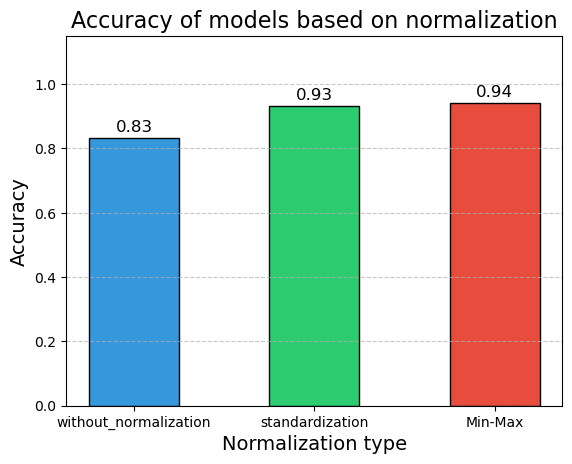
\includegraphics[keepaspectratio]{main_files/figure-pdf/cell-25-output-1.png}}

\begin{Shaded}
\begin{Highlighting}[]
\ImportTok{from}\NormalTok{ sklearn.metrics }\ImportTok{import}\NormalTok{ confusion\_matrix, ConfusionMatrixDisplay}
\NormalTok{confusionMatrixDT }\OperatorTok{=}\NormalTok{ metrics.confusion\_matrix(yval, y\_knn\_val)}
\NormalTok{fig, ax }\OperatorTok{=}\NormalTok{ plt.subplots()}
\NormalTok{custom\_order }\OperatorTok{=}\NormalTok{ [}\StringTok{\textquotesingle{}Good\textquotesingle{}}\NormalTok{, }\StringTok{\textquotesingle{}Moderate\textquotesingle{}}\NormalTok{, }\StringTok{\textquotesingle{}Poor\textquotesingle{}}\NormalTok{, }\StringTok{\textquotesingle{}Hazardous\textquotesingle{}}\NormalTok{]}

\NormalTok{confusionMatrixDT }\OperatorTok{=}\NormalTok{ confusion\_matrix(yval, y\_knn\_val, labels}\OperatorTok{=}\NormalTok{custom\_order)}

\NormalTok{disp }\OperatorTok{=}\NormalTok{ ConfusionMatrixDisplay(confusion\_matrix}\OperatorTok{=}\NormalTok{confusionMatrixDT,}
\NormalTok{                              display\_labels}\OperatorTok{=}\NormalTok{custom\_order)}
\NormalTok{disp.plot(ax}\OperatorTok{=}\NormalTok{ax, cmap}\OperatorTok{=}\StringTok{"viridis\_r"}\NormalTok{)}
\NormalTok{ax.set\_title(}\StringTok{"Confusion Matrix"}\NormalTok{, fontsize }\OperatorTok{=} \DecValTok{17}\NormalTok{)}
\NormalTok{ax.set\_xlabel(}\StringTok{"Predicted"}\NormalTok{, fontsize }\OperatorTok{=} \DecValTok{13}\NormalTok{)}
\NormalTok{ax.set\_ylabel(}\StringTok{"True"}\NormalTok{, fontsize }\OperatorTok{=} \DecValTok{13}\NormalTok{)}
\end{Highlighting}
\end{Shaded}

\begin{verbatim}
Text(0, 0.5, 'True')
\end{verbatim}

\pandocbounded{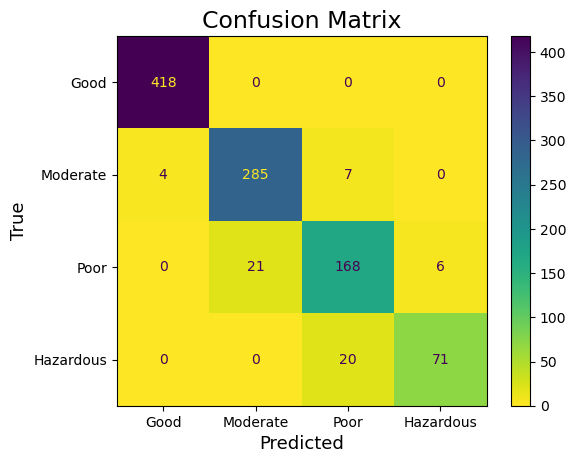
\includegraphics[keepaspectratio]{main_files/figure-pdf/cell-26-output-2.png}}

\subsection{Test accuracy}\label{test-accuracy}

Our model has 0.921 accuracy on test dateset, this is the accuracy that
we can expect on new data

\begin{Shaded}
\begin{Highlighting}[]
\NormalTok{scaler }\OperatorTok{=}\NormalTok{ MinMaxScaler()}
\NormalTok{Xtrain\_fit }\OperatorTok{=}\NormalTok{ scaler.fit\_transform(Xtrain)}
\NormalTok{Xtest\_fit }\OperatorTok{=}\NormalTok{ scaler.transform(Xtest)}

\NormalTok{clfKNN }\OperatorTok{=}\NormalTok{ KNeighborsClassifier(}\OperatorTok{**}\NormalTok{best\_params\_minmax)}
\NormalTok{clfKNN.fit(Xtrain\_fit, ytrain)}
\NormalTok{y\_knn\_val }\OperatorTok{=}\NormalTok{ clfKNN.predict(Xtest\_fit)}
\NormalTok{display(metrics.accuracy\_score(ytest, y\_knn\_val))}
\end{Highlighting}
\end{Shaded}

\begin{verbatim}
0.921
\end{verbatim}

\paragraph{Sources:}\label{sources}

\url{https://en.wikipedia.org/wiki/K-nearest_neighbors_algorithm}\strut \\
\url{https://www.kaggle.com/datasets/mujtabamatin/air-quality-and-pollution-assessment/data}




\end{document}
